\documentclass[11pt,a4paper]{article}

% ----- Basic packages -----
\usepackage[utf8]{inputenc}
\usepackage[T1]{fontenc}
\usepackage{lmodern}
\usepackage{geometry}
\geometry{margin=1in}

% ----- Math and symbols -----
\usepackage{amsmath, amssymb, amsfonts}
\usepackage{siunitx}
\sisetup{separate-uncertainty=true}

% ----- Graphics and tables -----
\usepackage{graphicx}
\usepackage{float}
\usepackage{booktabs}
\usepackage{array}
\usepackage{longtable}
\usepackage{caption}
\usepackage{subcaption}

% Optional: set common image search paths (adjust to your repo)
\graphicspath{{../out/}{../out_gaussian/}{../offaxis/}{../sweep_N/}{../sweep_lambda/}{../sweep_D2/}{../sweep_OD/}}

% ----- Links and references -----
\usepackage[hidelinks]{hyperref}
\usepackage{url}
\usepackage{cleveref}

% ----- Lists and spacing -----
\usepackage{enumitem}
\setlist{nosep}
\usepackage{titlesec}
\titlespacing*{\section}{0pt}{1.2em}{0.6em}
\titlespacing*{\subsection}{0pt}{1em}{0.4em}

% ----- Pandoc helper -----
\newcommand{\pandocbounded}[1]{#1}

% ----- (Optional) Map a few stray Unicode to ASCII if they appear -----
\DeclareUnicodeCharacter{2212}{-} % Unicode minus → hyphen
\DeclareUnicodeCharacter{2265}{$\ge$} % ≥
\DeclareUnicodeCharacter{2192}{$\to$} % →

% ----- Metadata -----
\title{Optical Simulation and PSF Analysis}
\author{Yuanhao Wang}
\date{\today}

\begin{document}
	\maketitle
	
	\section{Experiment}\label{experiment}
	
	For the evaluation of the results, we consider the Thorlabs LB1761 (a simple N-BK7 biconvex singlet lens) and perform a simulation using an f/8 aperture placed \SI{2}{\milli\meter} from the second lens surface.
	We map \([R1, T, R2, D2, OD]\) (mm) as:
	\textbf{R1 = 24.5}, \textbf{T = 9}, \textbf{R2 = -24.5}, \textbf{D2 = 22.2}, \textbf{OD = 3.175} (f/8).
	
	We only use \textbf{OD = 6.25 mm} for off-axis sweep and field\_grid sweep.
	
	We conducted the following experiments:
	\begin{itemize}
		\item Function test
		\item Layout \& Ray visualization
		\item Best focus estimation
		\item Sampling number (N) sweep
		\item Wavelength (\(\lambda\)) sweep
		\item Through-focus (D2) sweep
		\item Aperture sweep (OD)
		\item Off-axis sweep
	\end{itemize}
	
	Further, we consider a double-Gaussian lens \href{https://patents.google.com/patent/US2532751}{US2532751A}, and conducted:
	\begin{itemize}
		\item Wavelength (\(\lambda\)) sweep
		\item Off-axis sweep
	\end{itemize}
	
	\subsubsection*{Function Test}\label{function-test}
	
	Function tests are in \href{../tests/test_geo.py}{\texttt{test\_geo.py}} and \href{../tests/test_ray_tracing.py}{\texttt{test\_ray\_tracing.py}}.
	
	\paragraph{Lens layout.}%
	\pandocbounded{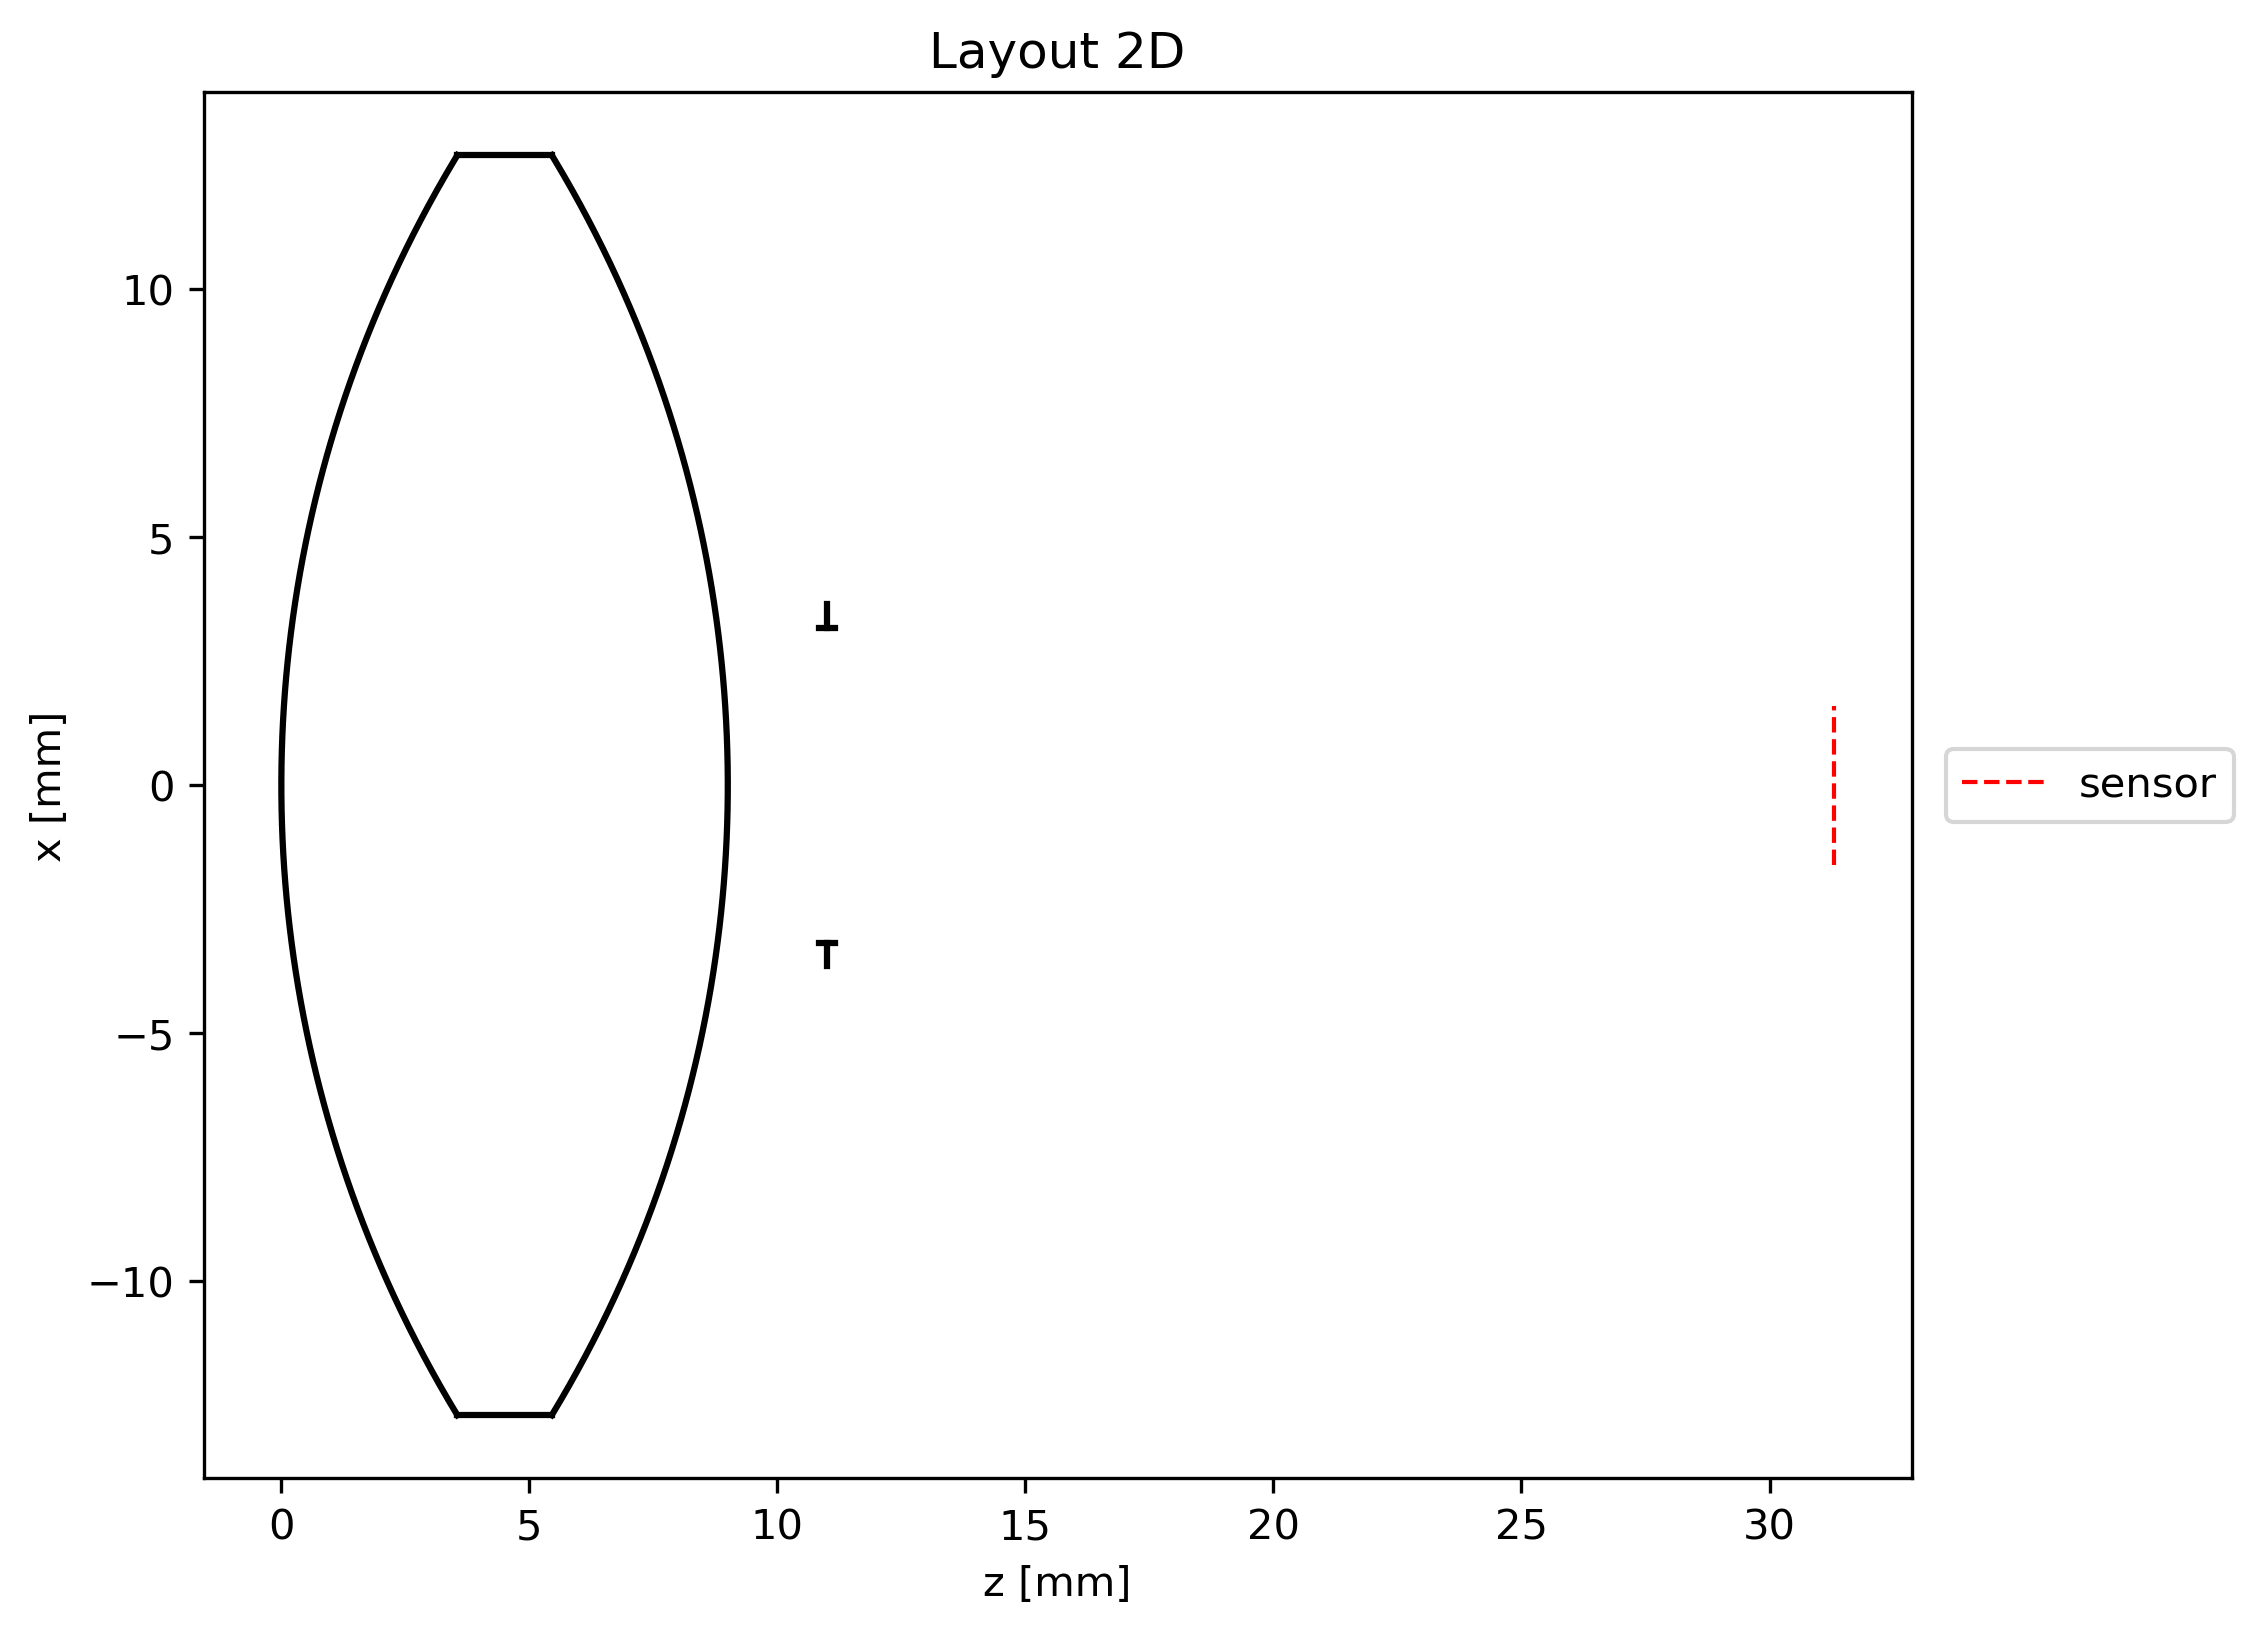
\includegraphics[width=\linewidth,keepaspectratio]{biconvex_layout.png}}
	
	\paragraph{Ray tracing.}%
	\pandocbounded{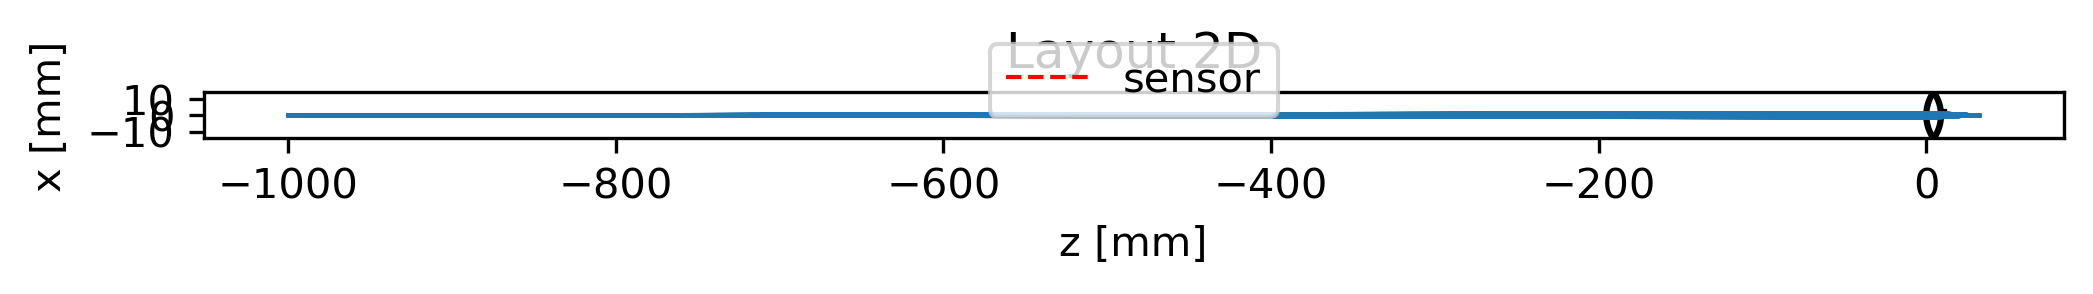
\includegraphics[width=\linewidth,keepaspectratio]{biconvex_rays.png}}
	
	\subsubsection*{PSF Examples}\label{psf-examples}
	
	After optimization, placing the sensor (mm) at the following distances \emph{after the aperture} yields the best focus:
	
	\begin{table}[H]
		\centering
		\caption{Best focus distance vs. aperture}
		\begin{tabular}{lcccc}
			\toprule
			\textbf{Aperture (mm)} & \textbf{1.6 (f/16)} & \textbf{3.175 (f/8)} & \textbf{6.35 (f/4)} & \textbf{12.7 (f/2)} \\
			\midrule
			\textbf{Best Focus Distance (mm)} & 20.55 & 20.5 & 20.3 & 18.7 \\
			\bottomrule
		\end{tabular}
	\end{table}
	
	\textbf{Observation}: The best sensor-to-aperture distance varies slightly with aperture size, shifting from \SI{20.55}{mm} at f/16 to \SI{18.7}{mm} at f/2 due to increased spherical aberration at larger apertures.
	
	\begin{figure}[H]
		\centering
		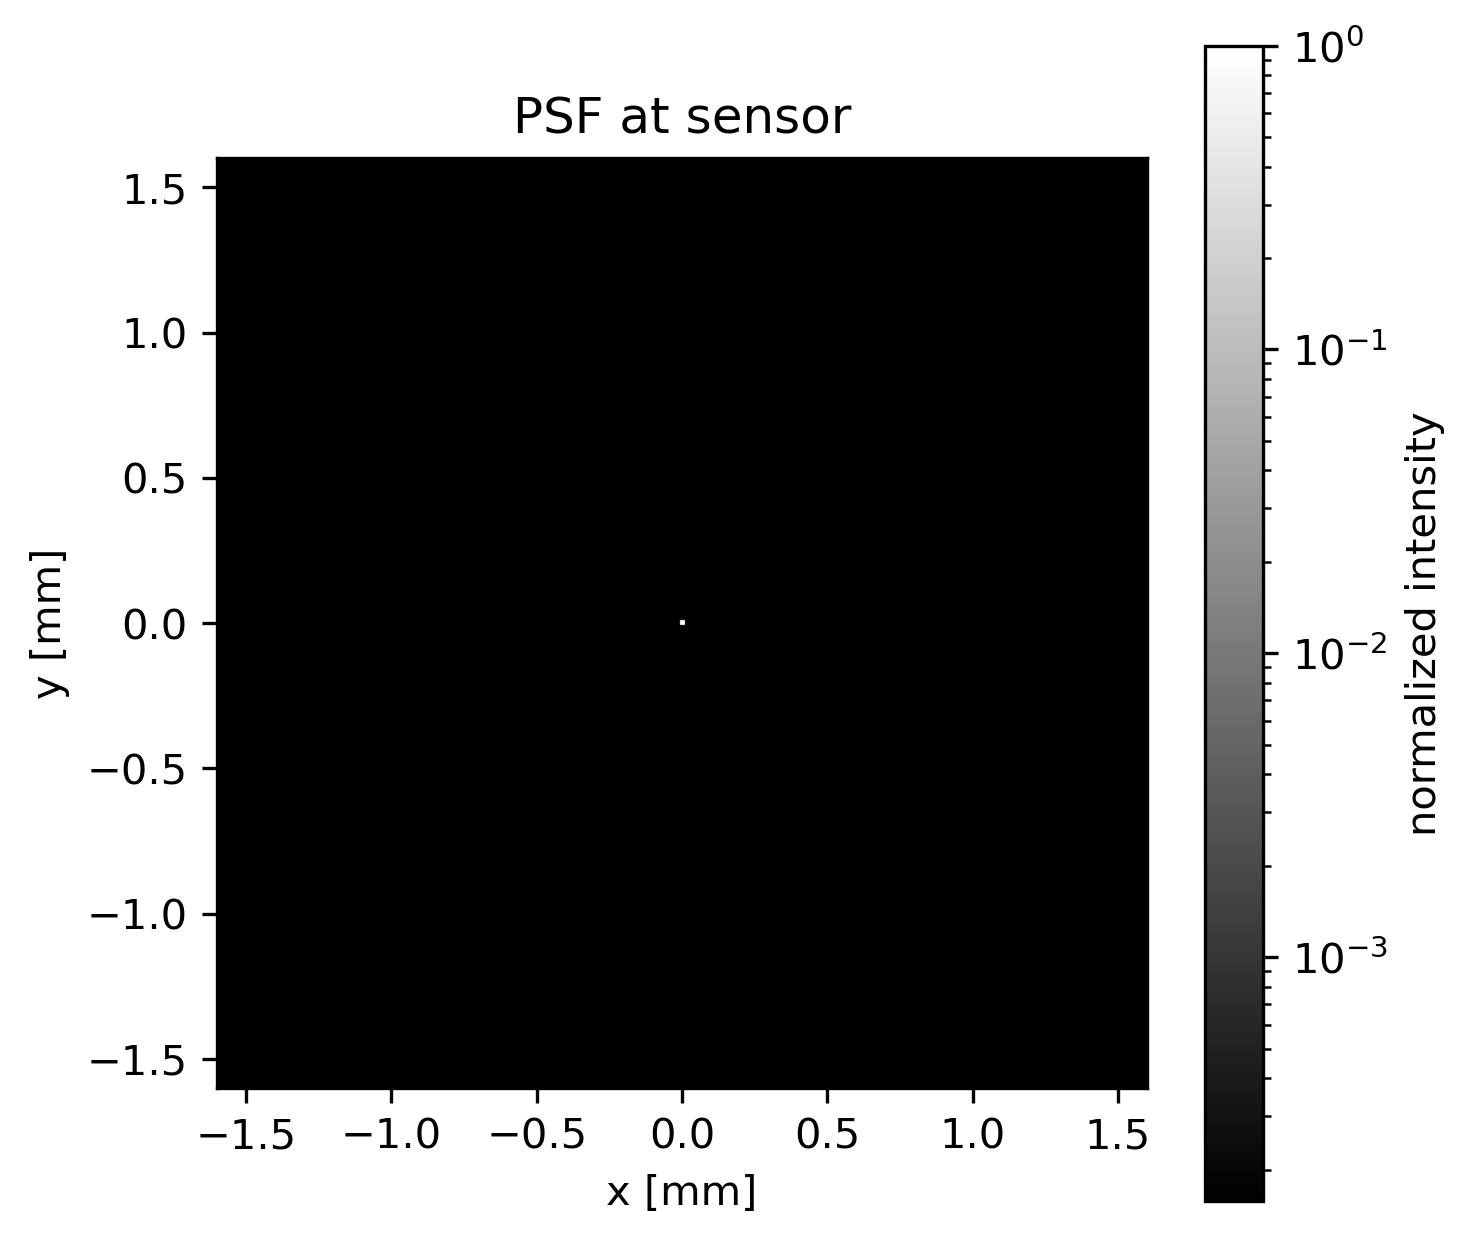
\includegraphics[width=\linewidth]{biconvex_psf_log.png}
		\caption{PSF (log scale) at best focus.}
	\end{figure}
	
	\subsubsection*{N-sweep (sampling)}\label{n-sweep-sampling}
	
	We swept \(N \in \{50, 100, 400, 1600, 3200, 6400\}\) and computed metrics vs. \(N\).
	To probe focus sensitivity, we also used a larger aperture \(\mathrm{OD} = \SI{6.35}{mm}\) and repeated the PSF analysis.
	
	Illustrations for \(N=\{50, 400, 3200\}\) are shown below (more in the \href{../out/sweep_N}{folder}):
	
	\begin{table}[H]
		\centering
		\begin{tabular}{>{\centering\arraybackslash}m{0.31\linewidth} >{\centering\arraybackslash}m{0.31\linewidth} >{\centering\arraybackslash}m{0.31\linewidth}}
			\toprule
			\textbf{N = 50} & \textbf{N = 400} & \textbf{N = 3200}\\
			\midrule
			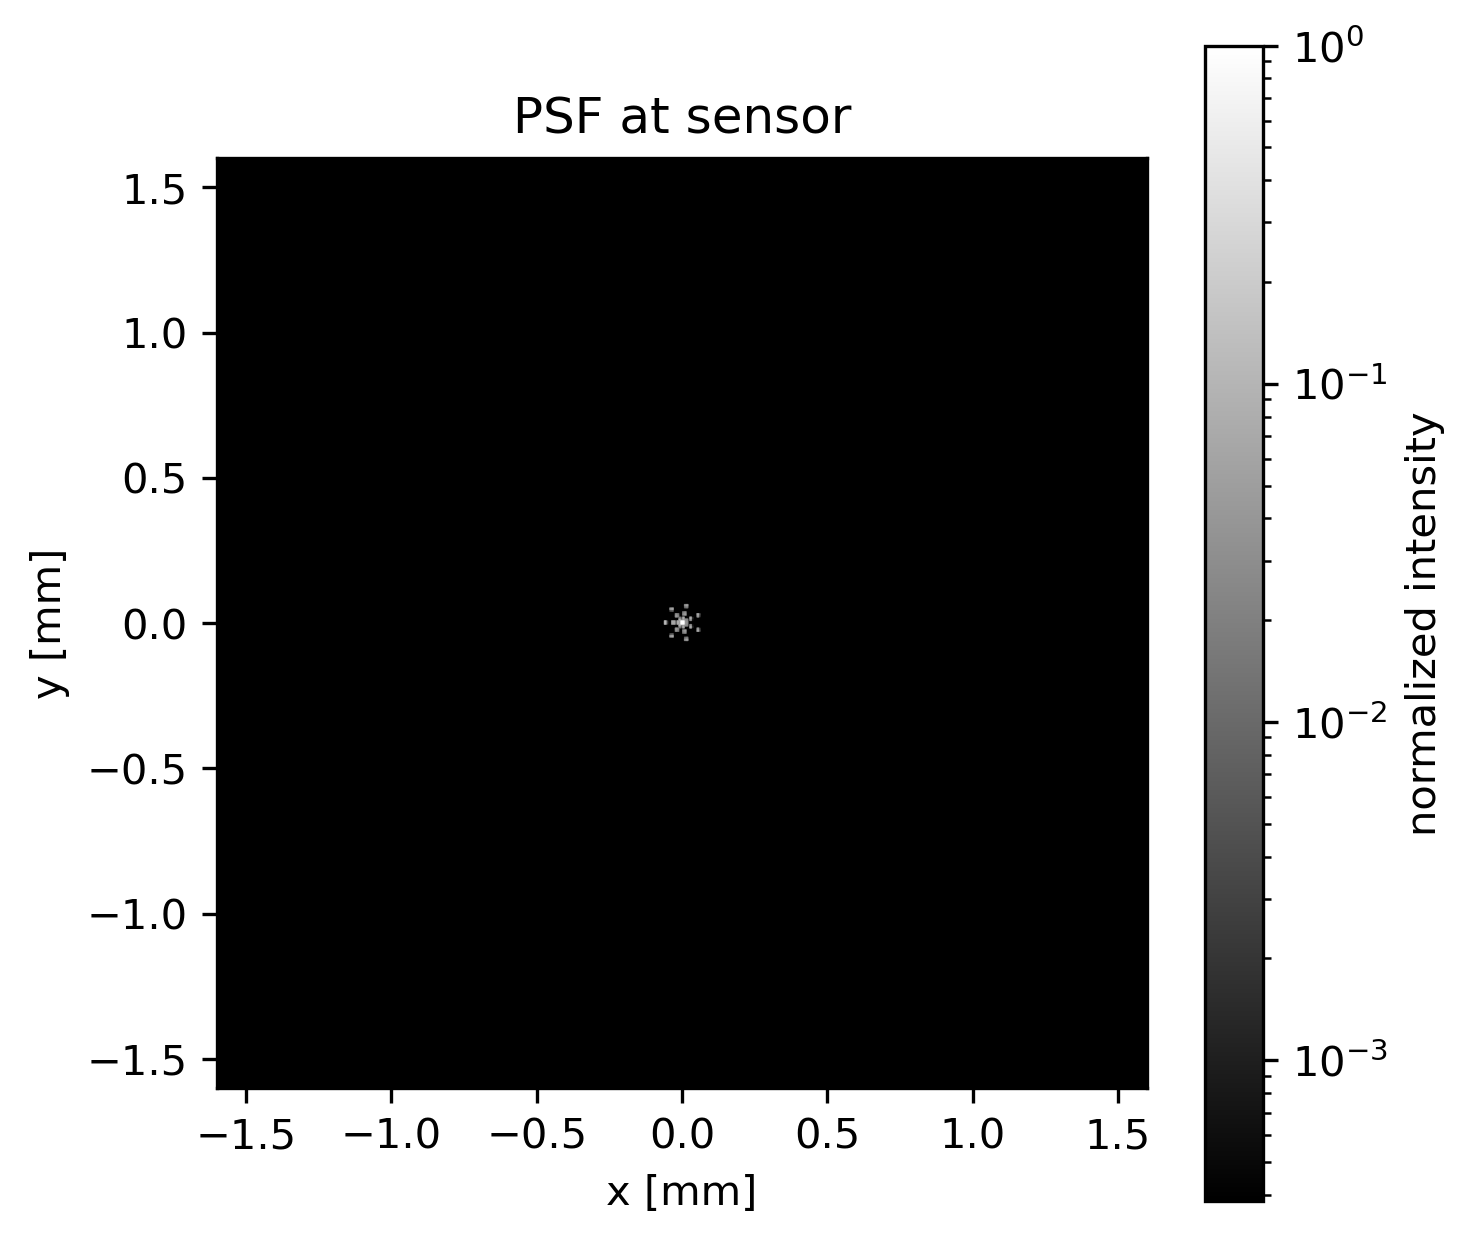
\includegraphics[width=\linewidth,keepaspectratio]{sweep_N/biconvex_psf_50_log.png} &
			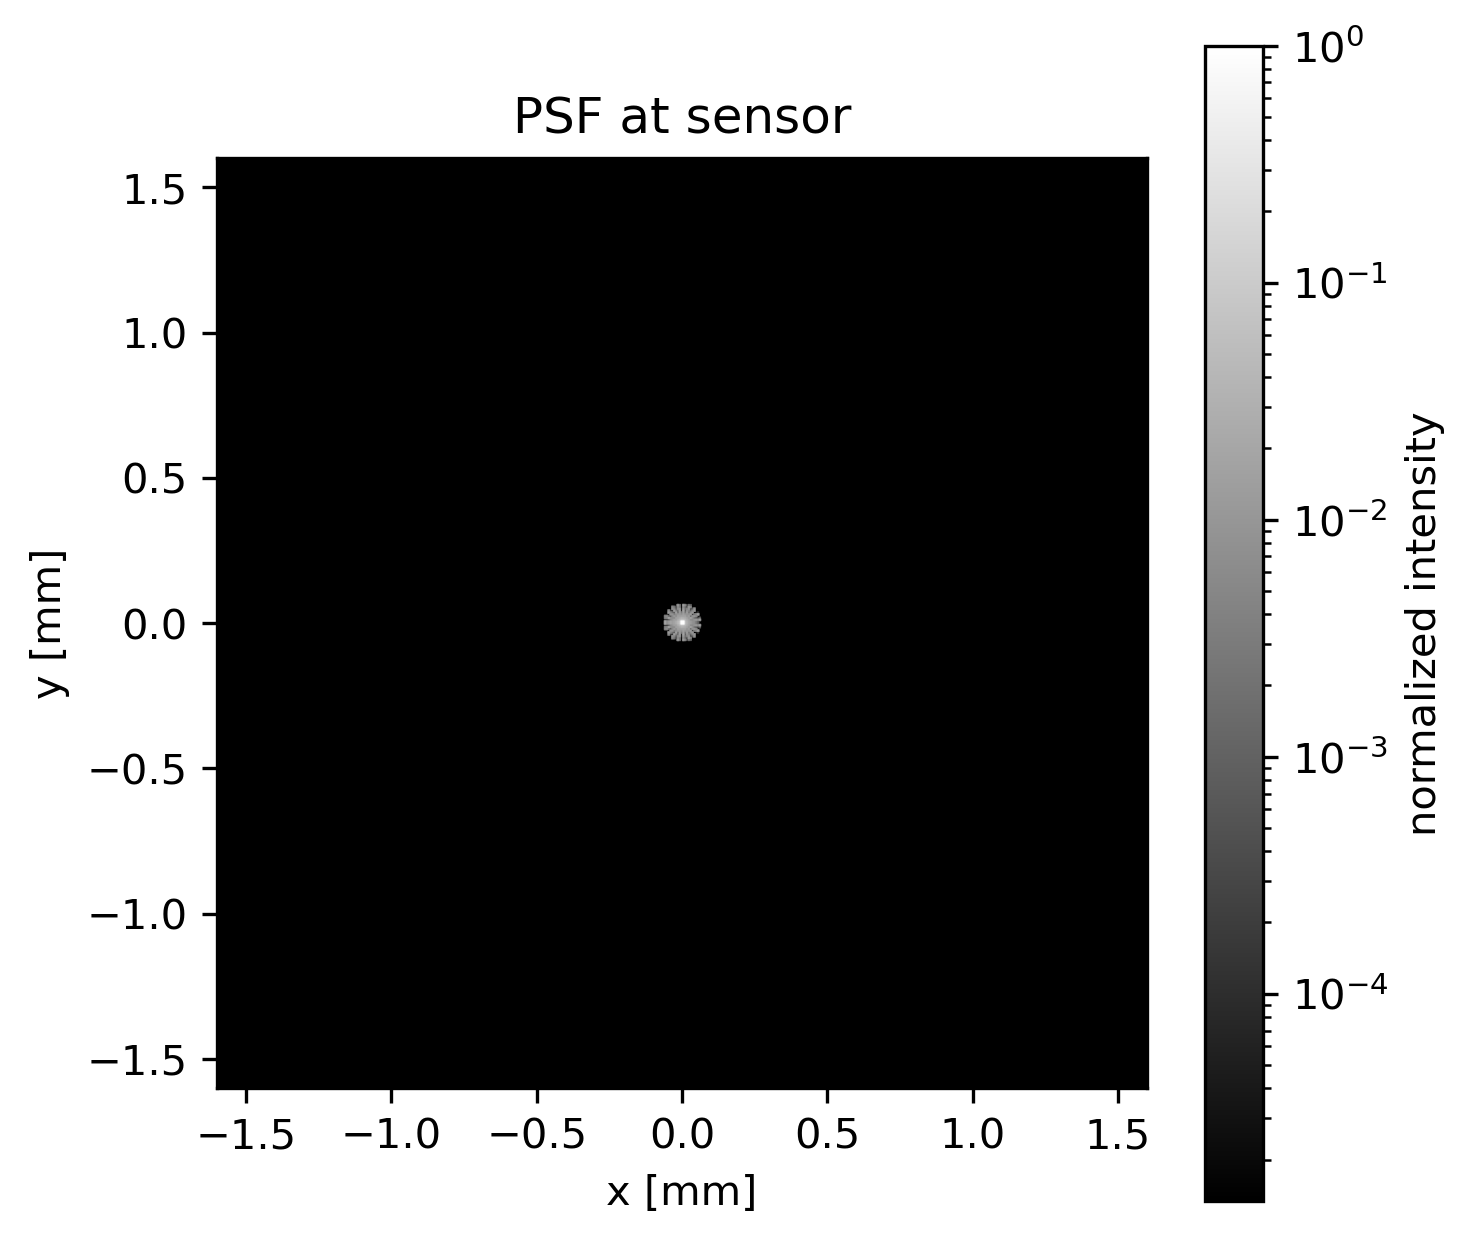
\includegraphics[width=\linewidth,keepaspectratio]{sweep_N/biconvex_psf_400_log.png} &
			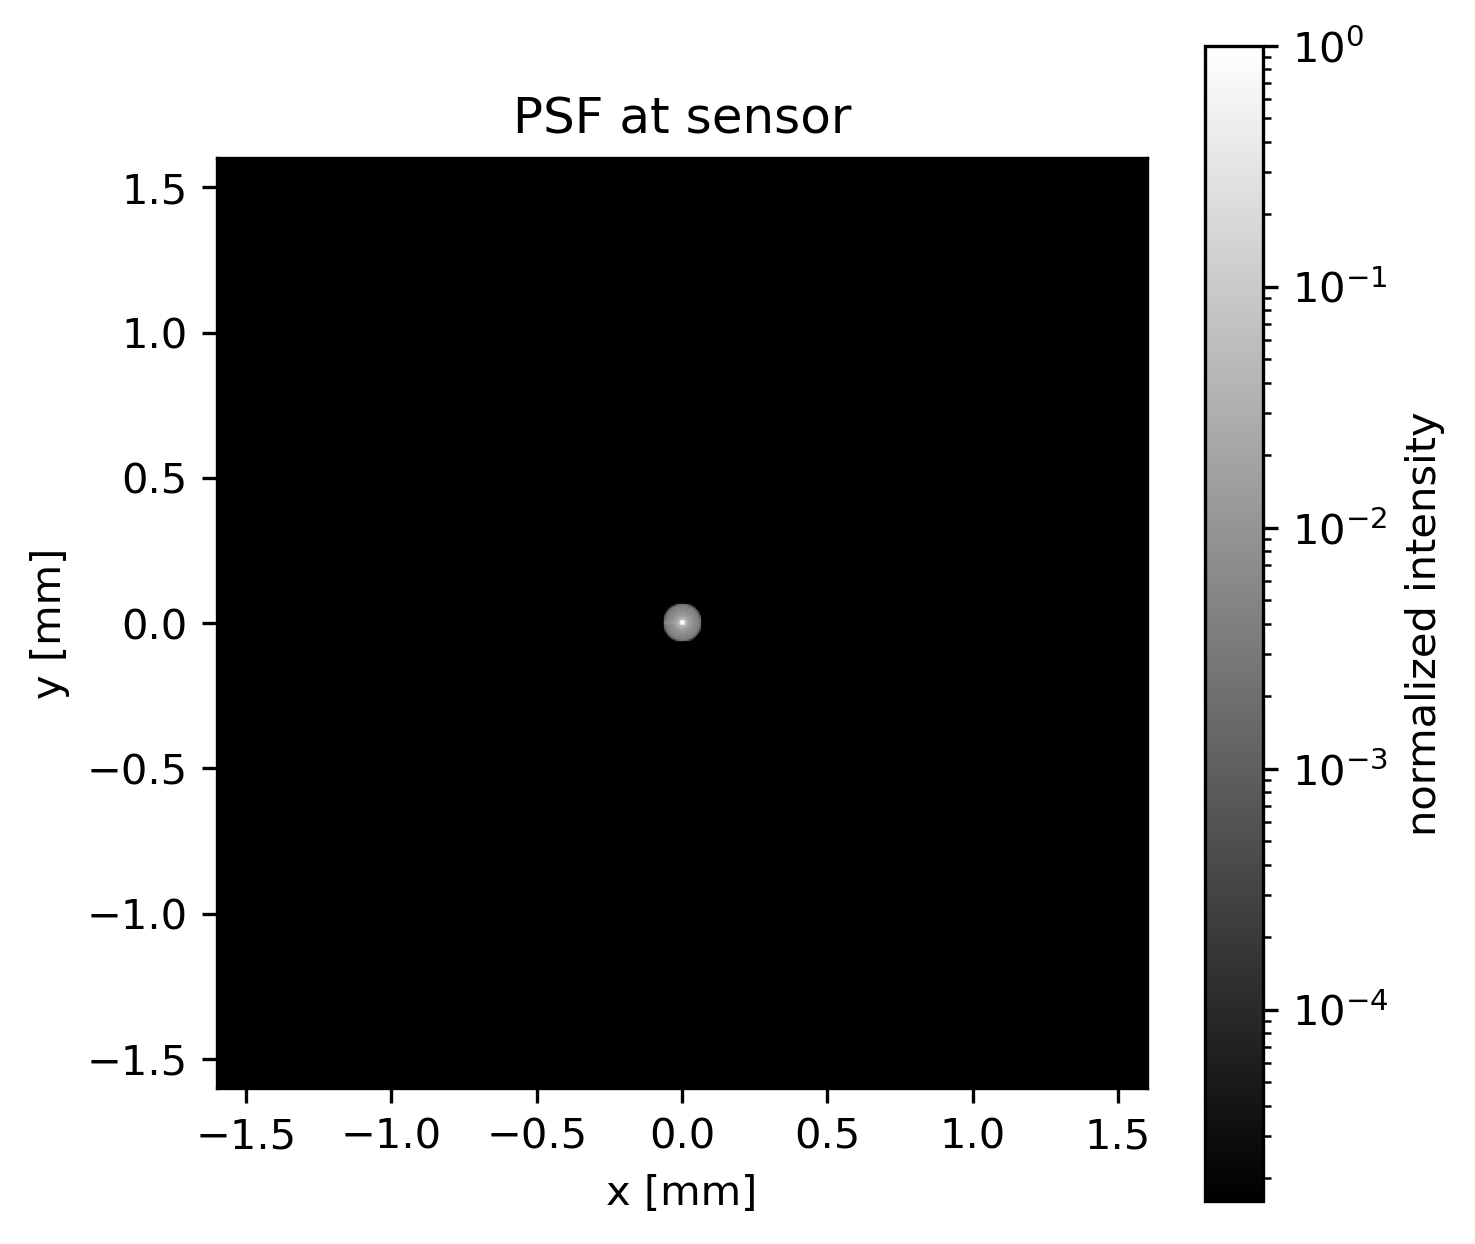
\includegraphics[width=\linewidth,keepaspectratio]{sweep_N/biconvex_psf_3200_log.png} \\
			\bottomrule
		\end{tabular}
		\caption{PSF snapshots vs. sampling count \(N\).}
	\end{table}
	
	EE50 and RMS metrics are recorded in \href{../out/sweep_N/metrics.csv}{\texttt{metrics.csv}} and plotted in:
	\begin{figure}[H]
		\centering
		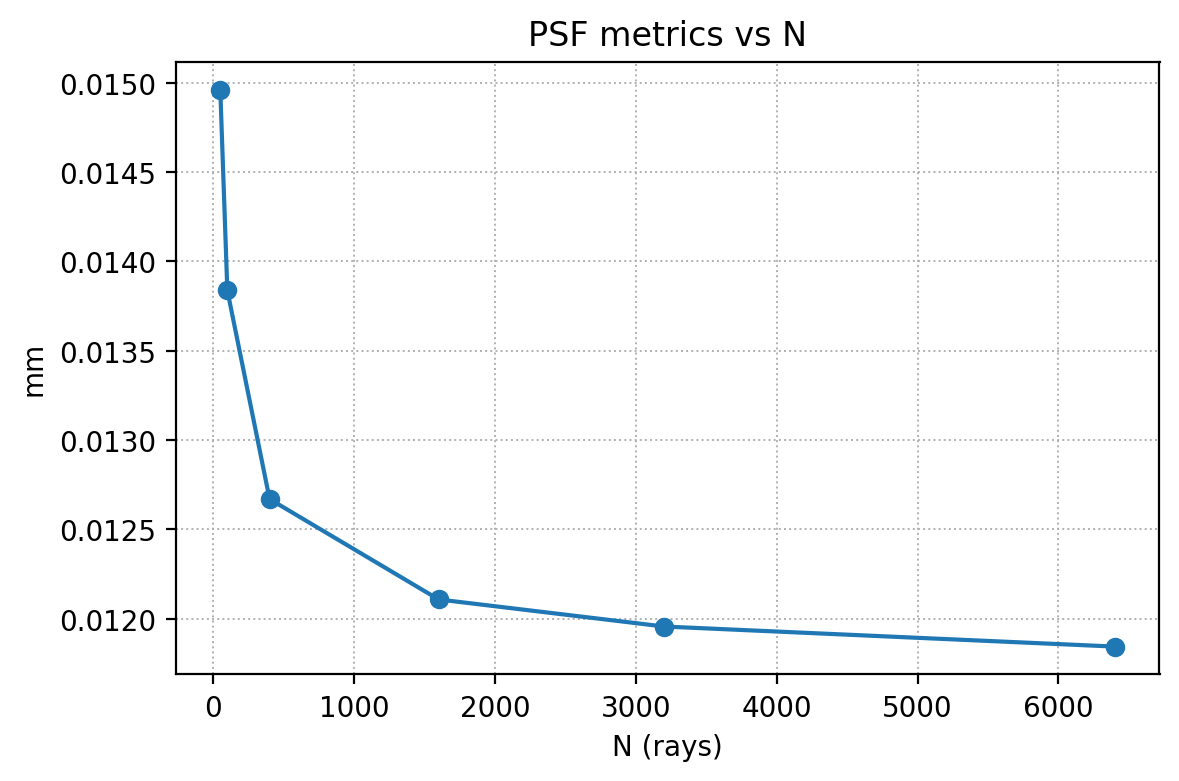
\includegraphics[width=\linewidth]{sweep_N/metrics_vs_N.png}
		\caption{Metrics vs. \(N\).}
	\end{figure}
	
	\textbf{Observation}: The convergence begins around \(N \ge 1600\), where RMS values stabilize to \(\sim 0.045\,\mathrm{mm}\) and \(\sim 0.021\,\mathrm{mm}\), indicating sufficient ray sampling density. We choose \(N=3200\) for the remaining experiments.
	
	\subsubsection*{Wavelength Sweep}\label{wavelength-sweep}
	
	We sweep \(\lambda \in \{430, 520, 610\}\,\mathrm{nm}\) (within the visible range):
	
	\begin{table}[H]
		\centering
		\begin{tabular}{>{\centering\arraybackslash}m{0.31\linewidth} >{\centering\arraybackslash}m{0.31\linewidth} >{\centering\arraybackslash}m{0.31\linewidth}}
			\toprule
			\(\lambda=\) \SI{430}{nm} & \(\lambda=\) \SI{520}{nm} & \(\lambda=\) \SI{610}{nm} \\
			\midrule
			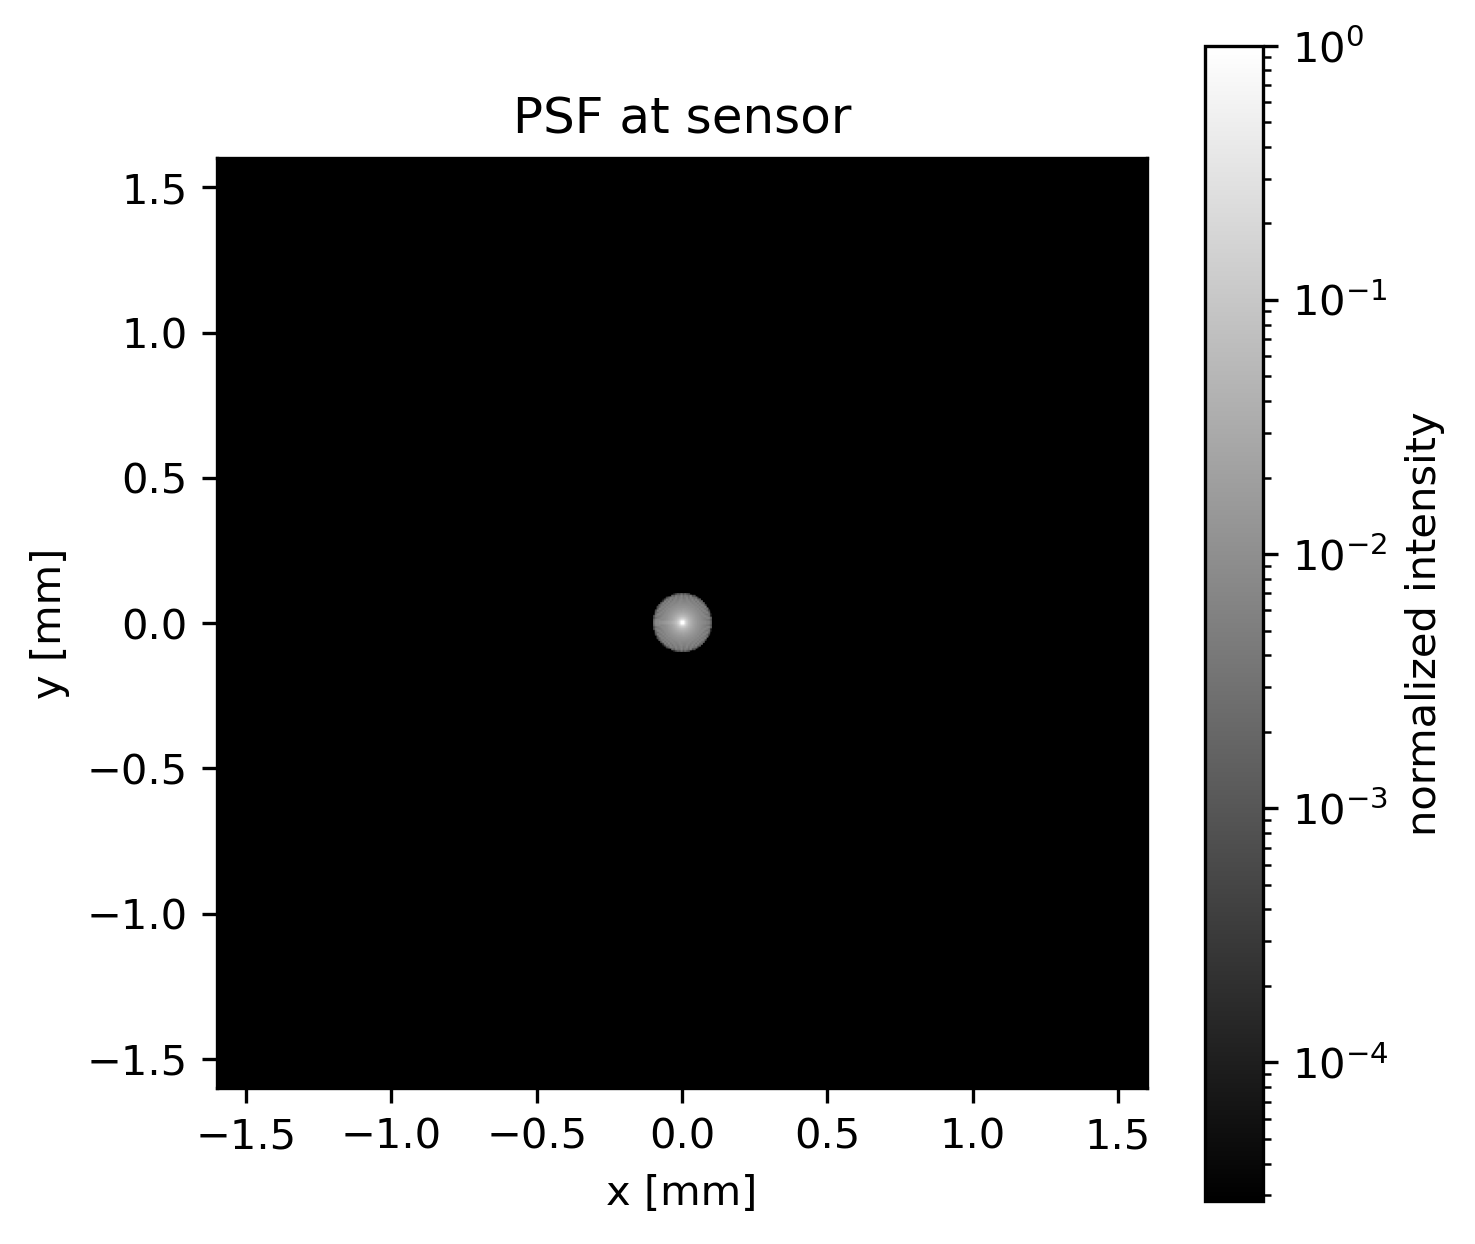
\includegraphics[width=\linewidth,keepaspectratio]{sweep_lambda/biconvex_psf_430_log.png} &
			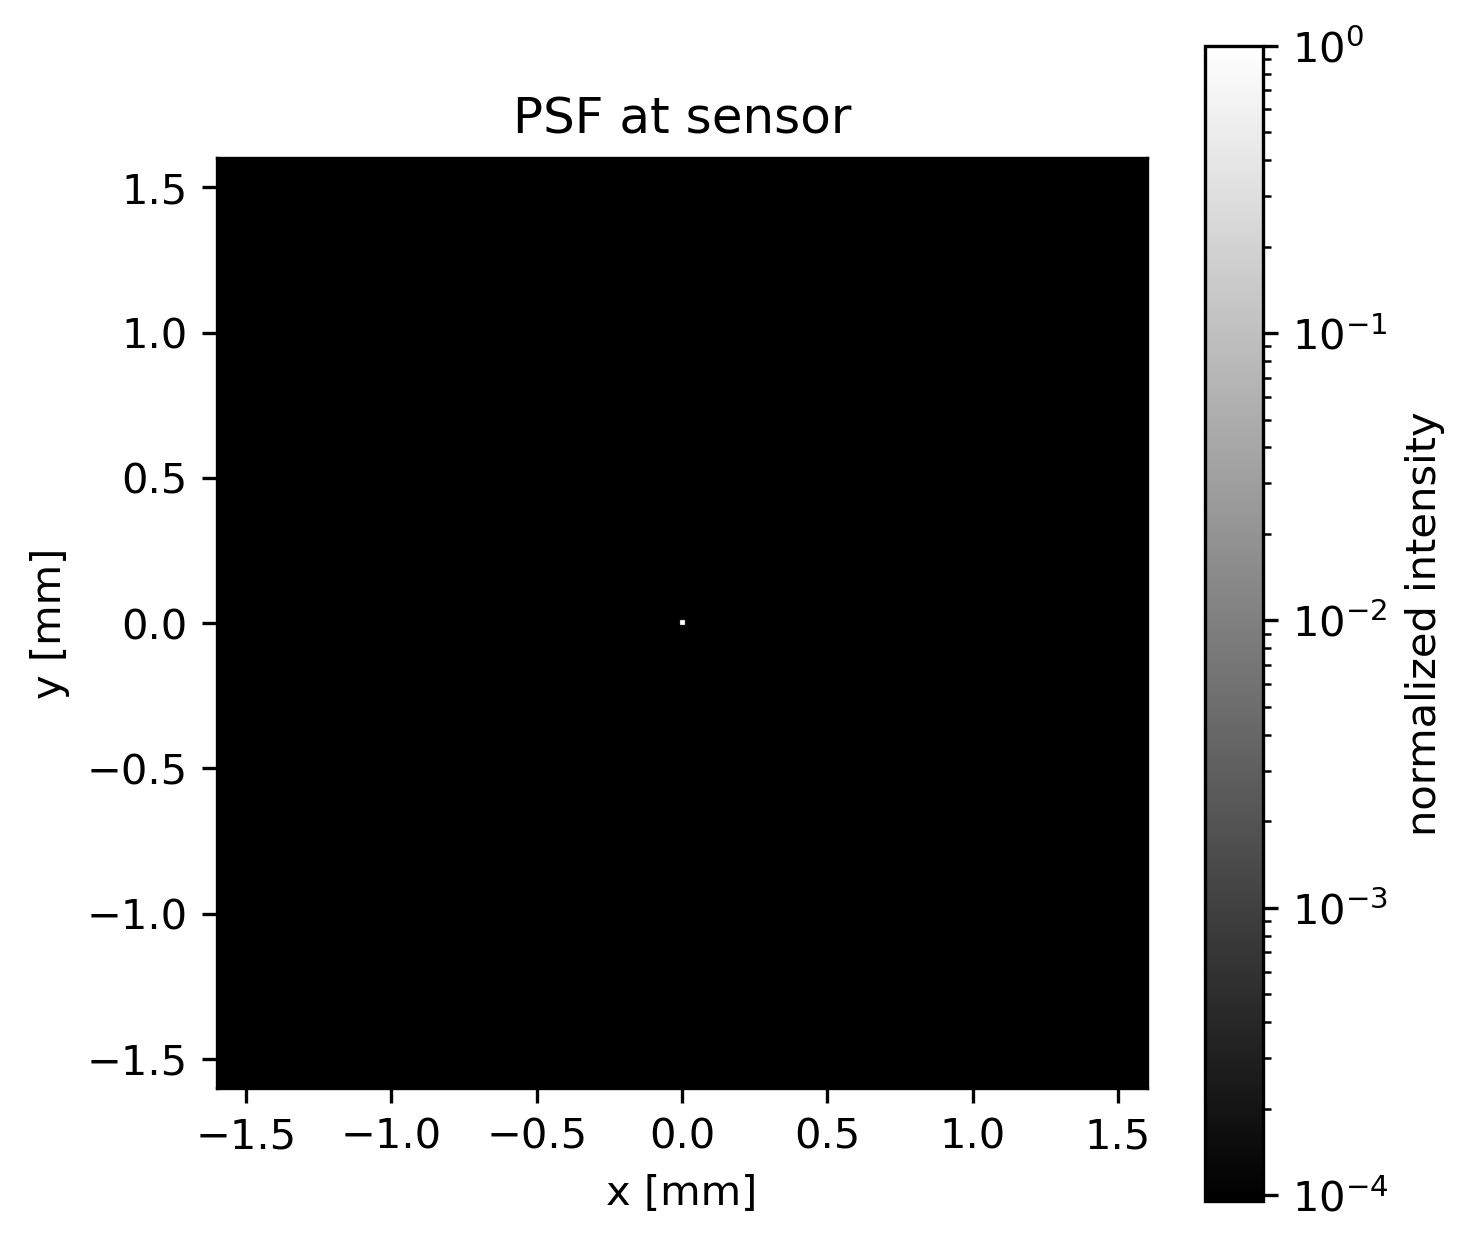
\includegraphics[width=\linewidth,keepaspectratio]{sweep_lambda/biconvex_psf_520_log.png} &
			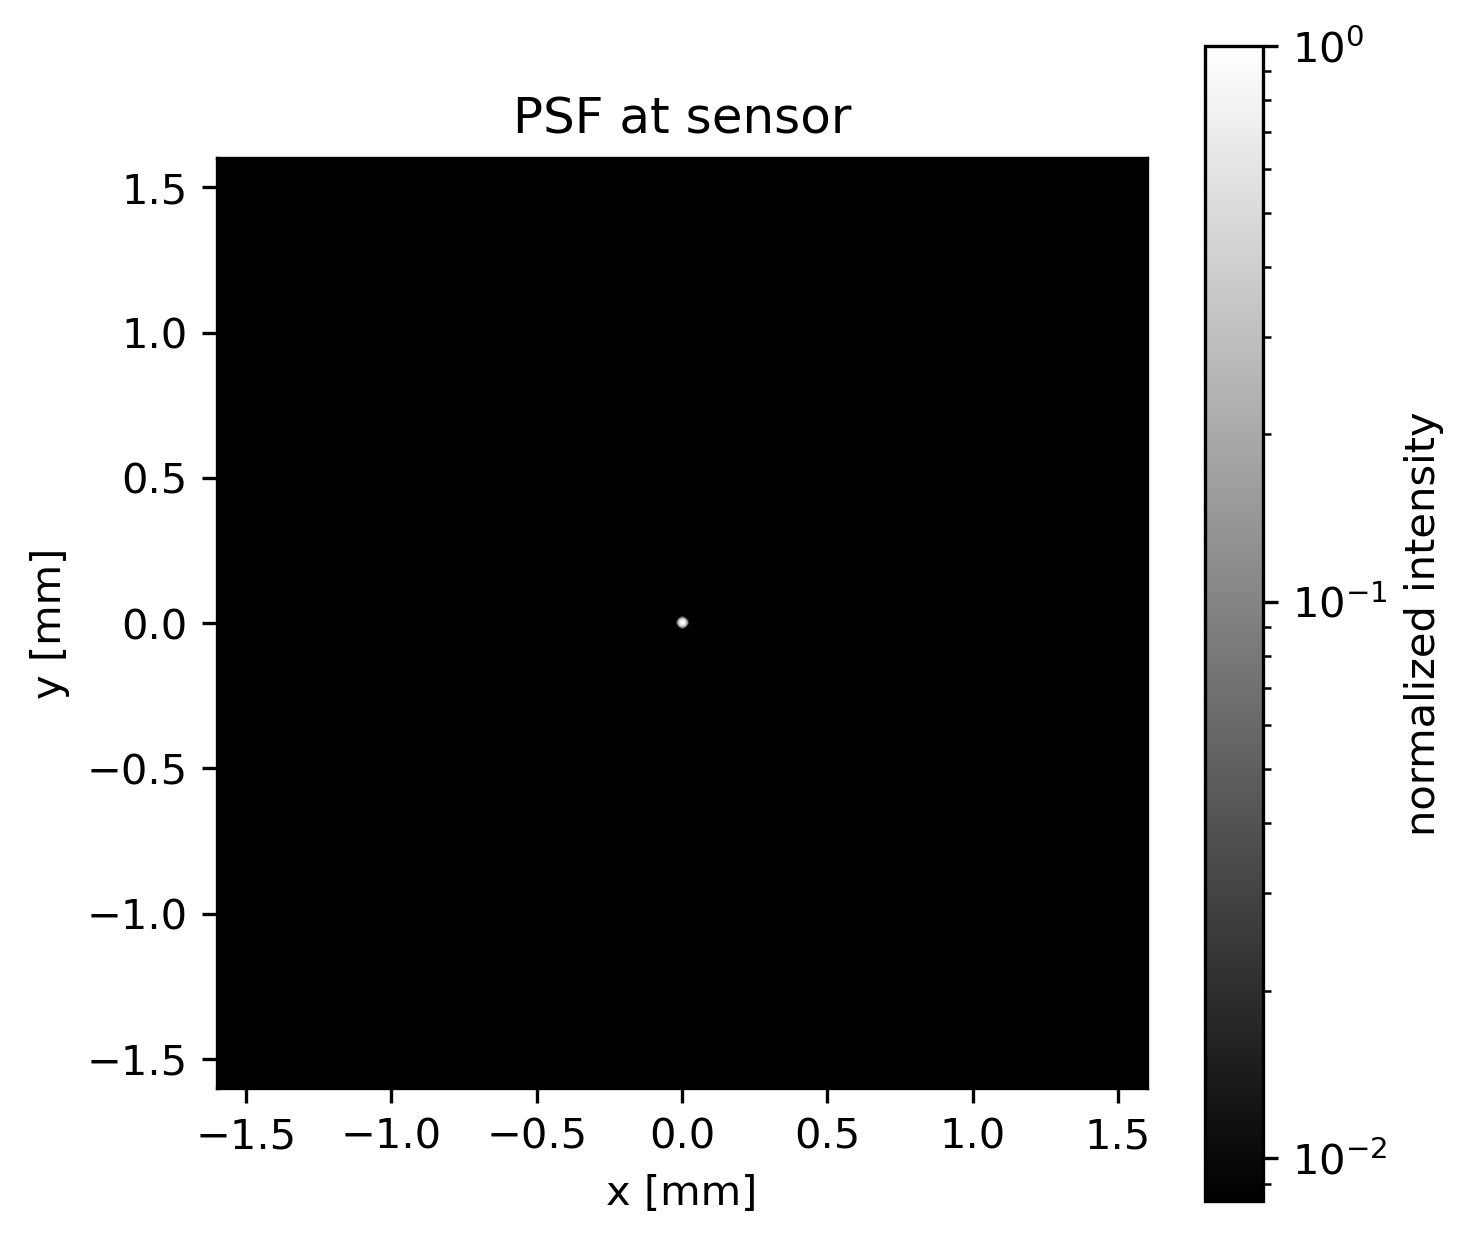
\includegraphics[width=\linewidth,keepaspectratio]{sweep_lambda/biconvex_psf_610_log.png} \\
			\bottomrule
		\end{tabular}
		\caption{PSF vs. wavelength.}
	\end{table}
	
	Metrics are in \href{../out/sweep_lambda/metrics.csv}{\texttt{metrics.csv}}; plot:
	\begin{figure}[H]
		\centering
		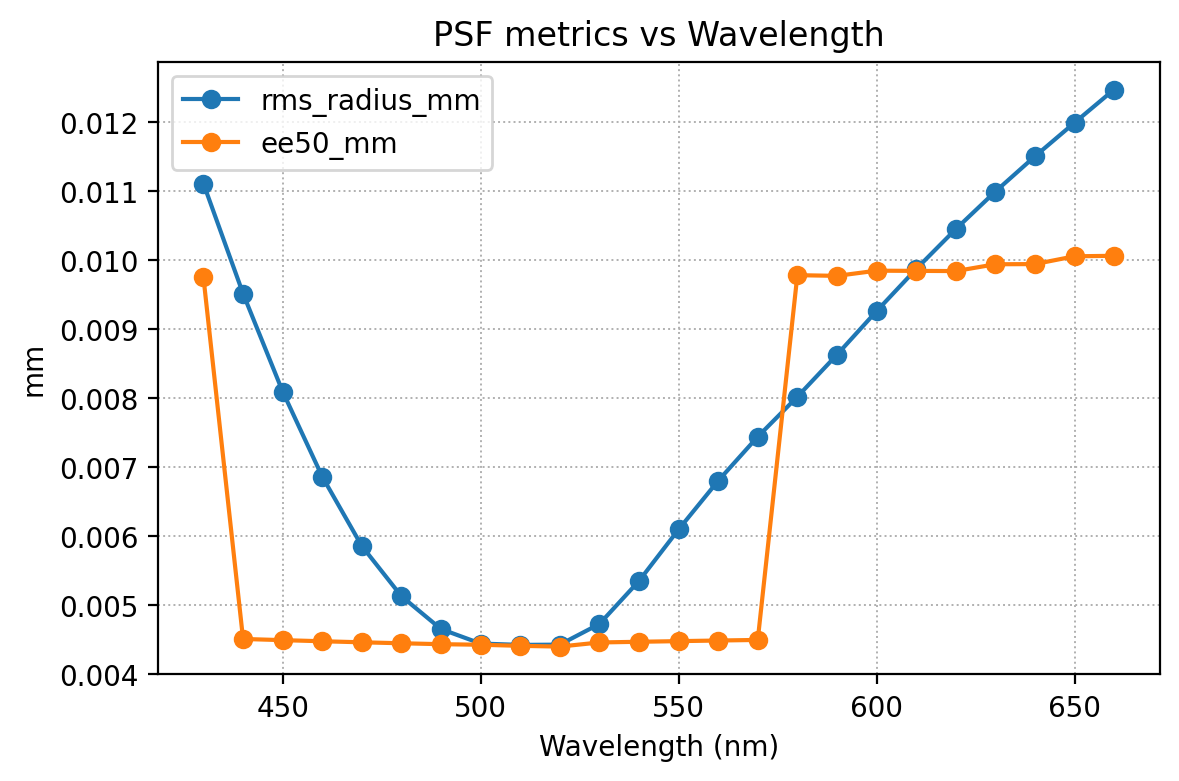
\includegraphics[width=\linewidth]{sweep_lambda/metrics_vs_lambda_nm.png}
		\caption{Metrics vs. wavelength.}
	\end{figure}
	
	\textbf{Observation}: With BK7 dispersion enabled, the smallest PSF occurs near \(\sim\) \SI{500}{nm} and grows toward both spectral ends (chromatic focus shift).
	
	\subsubsection*{Through-focus (D2 sweep)}\label{through-focus-d2-sweep}
	
	We sweep \(D_2 \in [19.5, 21.5]\ \mathrm{mm}\) (sampling 13 steps). The best focus is at \SI{20.5}{mm}.
	
	\begin{figure}[H]
		\centering
		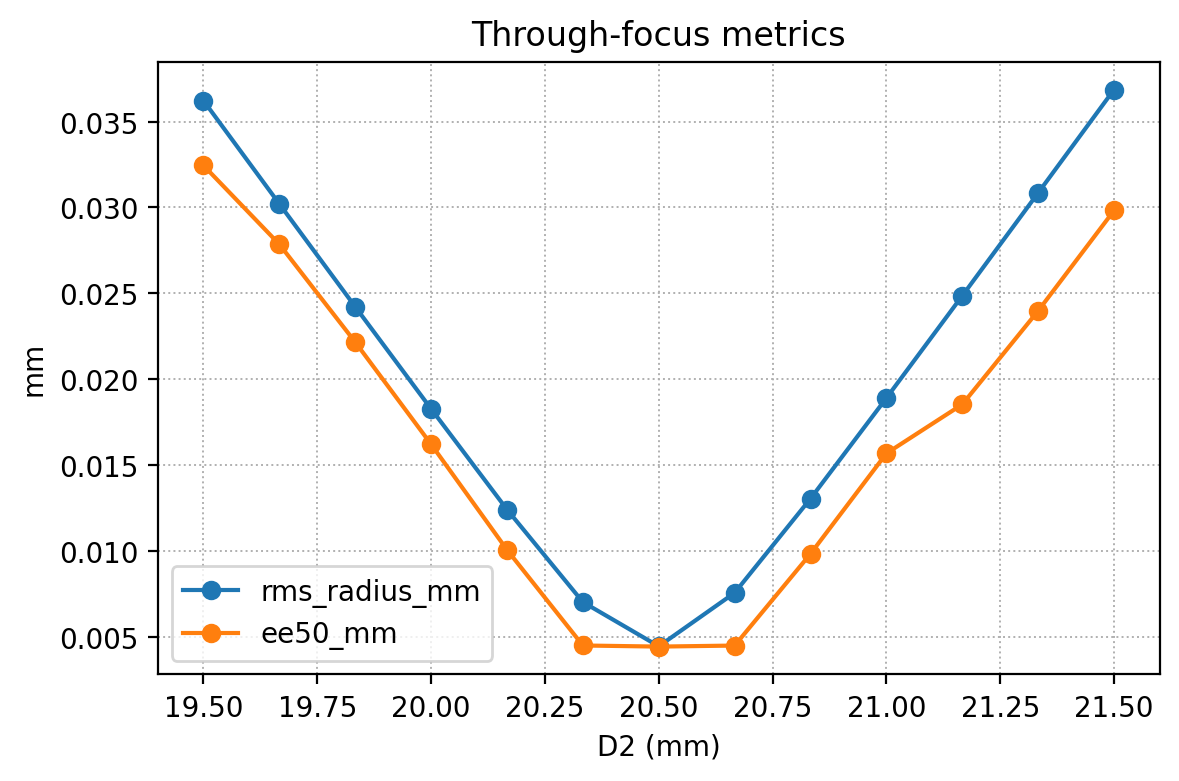
\includegraphics[width=\linewidth]{sweep_D2/metrics_vs_D2.png}
		\caption{Metrics vs. \(D_2\) (through-focus sweep).}
	\end{figure}
	
	\textbf{Observation}: Moving away from \SI{20.5}{mm} (e.g., toward 20.33 or 20.66) increases RMS and EE50 smoothly; the curve is slightly asymmetric due to real lens aberrations.
	
	\subsubsection*{Aperture Sweep (OD)}\label{aperture-sweep-od}
	
	We sweep \(\mathrm{OD} \in \{1.5875\ \mathrm{mm}\ (f/16),\ 3.175\ \mathrm{mm}\ (f/8),\ 6.35\ \mathrm{mm}\ (f/4),\ 12.7\ \mathrm{mm}\ (f/2)\}\).
	
	\begin{figure}[H]
		\centering
		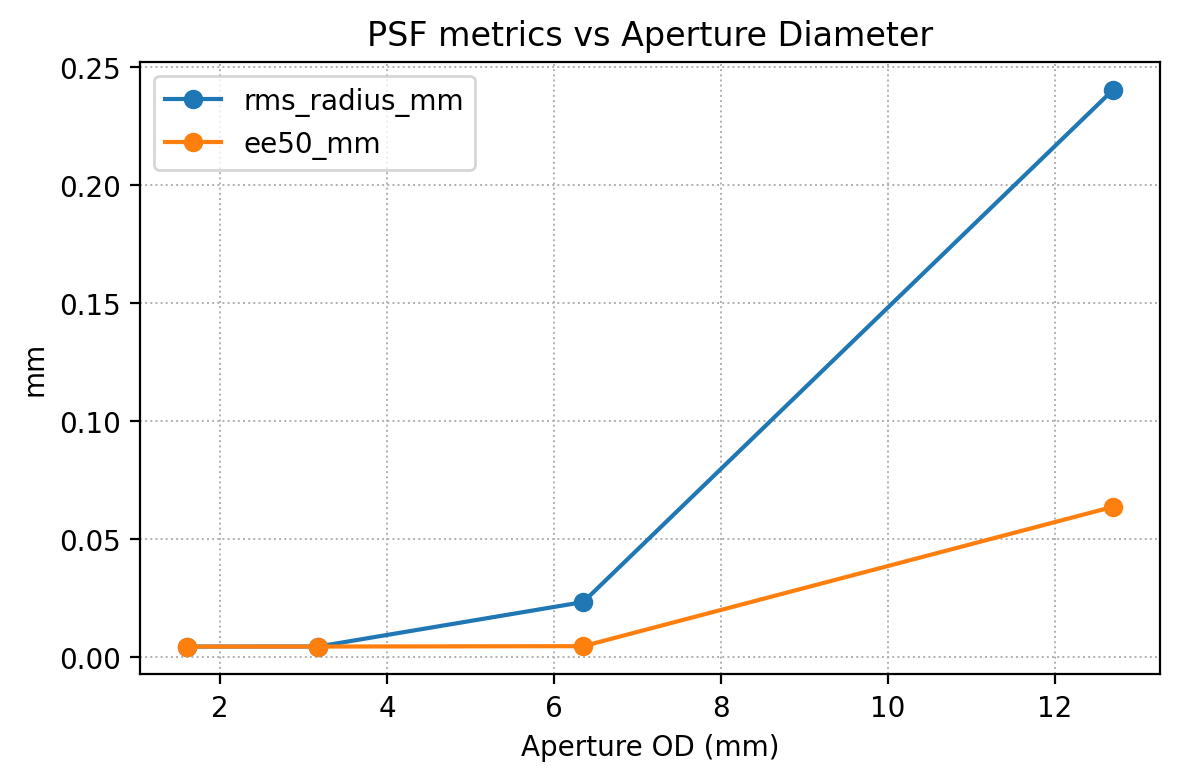
\includegraphics[width=\linewidth]{sweep_OD/metrics_vs_OD.png}
		\caption{Metrics vs. aperture (OD).}
	\end{figure}
	
	\textbf{Observation}: As aperture increases from $\sim$1.6 to {12.7}{mm}, the PSF core (EE50) stays nearly constant at small--moderate apertures, while the halo (RMS) grows; at the largest aperture both EE50 and RMS increase noticeably. The sharpest results occur near smaller apertures ($\sim$1.6--3.2 mm).
	
	\subsubsection*{Off-axis sweep}\label{off-axis-sweep}
	
	We consider \(\mathrm{OD}=\SI{6.35}{mm}\ (f/4)\) and field offsets \(-35, 0, 35\ \mathrm{mm}\):
	
	\begin{table}[H]
		\centering
		\begin{tabular}{>{\centering\arraybackslash}m{0.31\linewidth} >{\centering\arraybackslash}m{0.31\linewidth} >{\centering\arraybackslash}m{0.31\linewidth}}
			\toprule
			Off-axis = \(-\)35 mm & Off-axis = 0 mm & Off-axis = 35 mm \\
			\midrule
			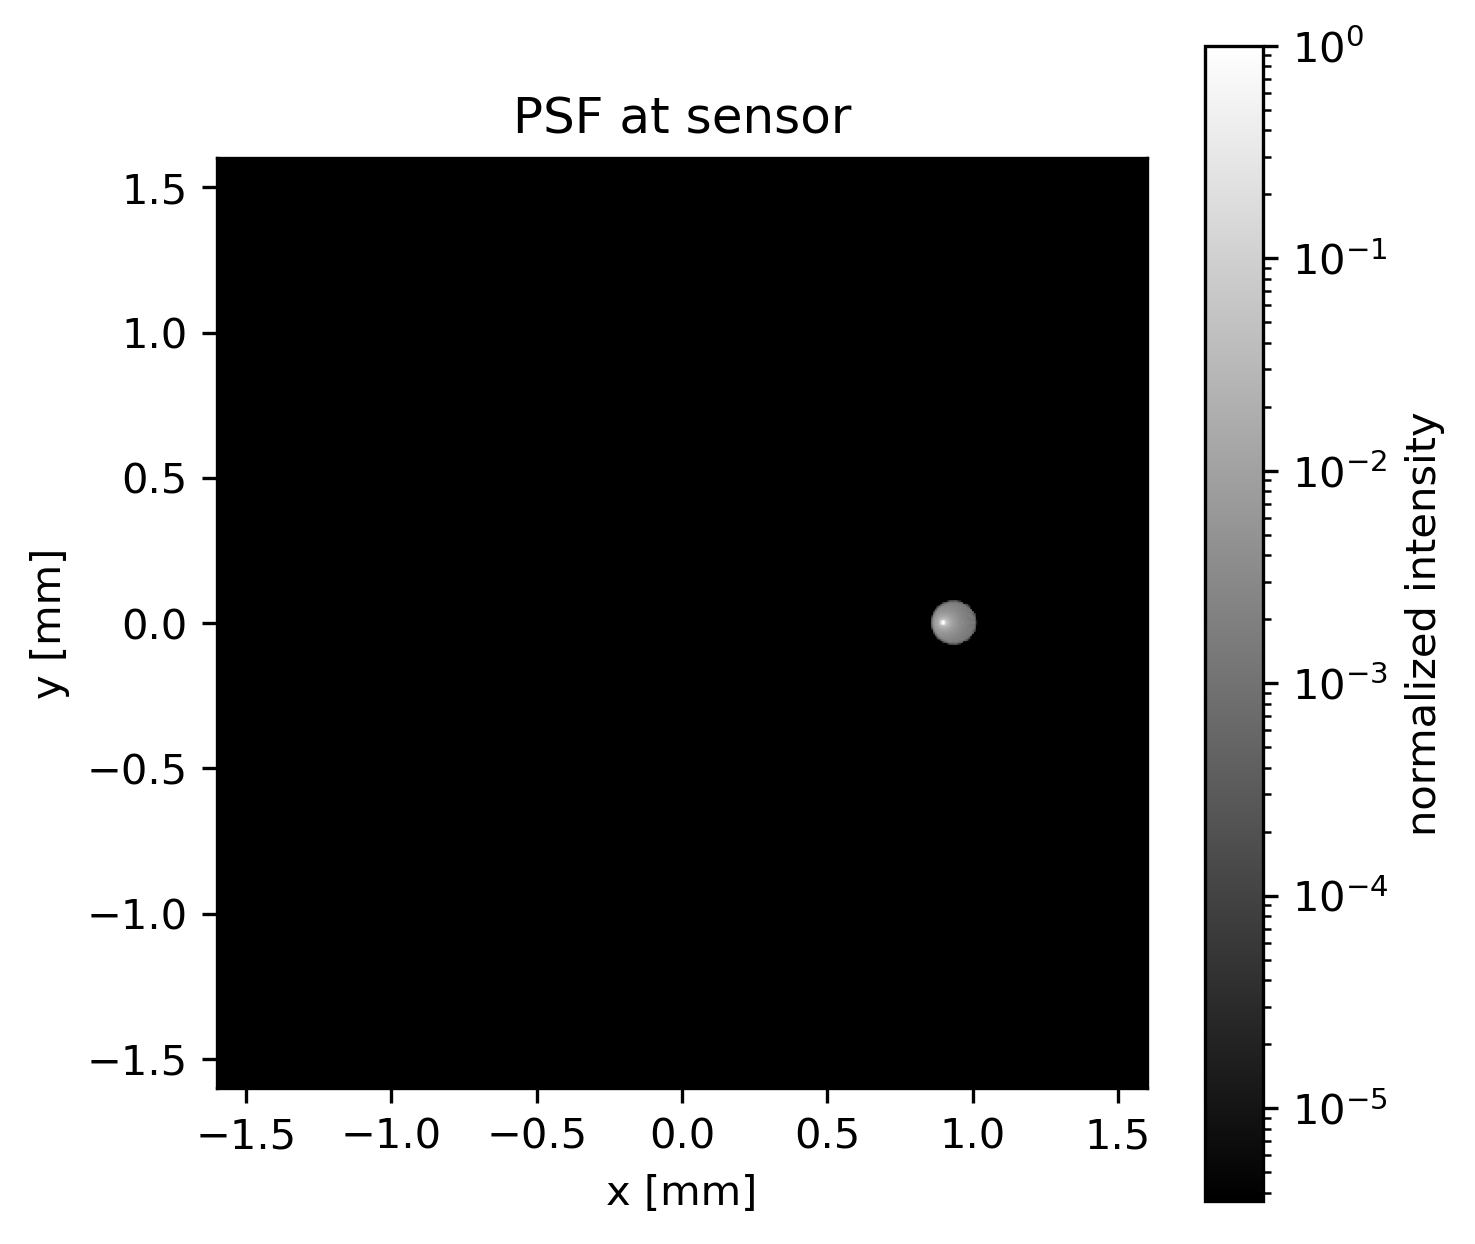
\includegraphics[width=\linewidth,keepaspectratio]{offaxis/biconvex_psf_-35.00_log.png} &
			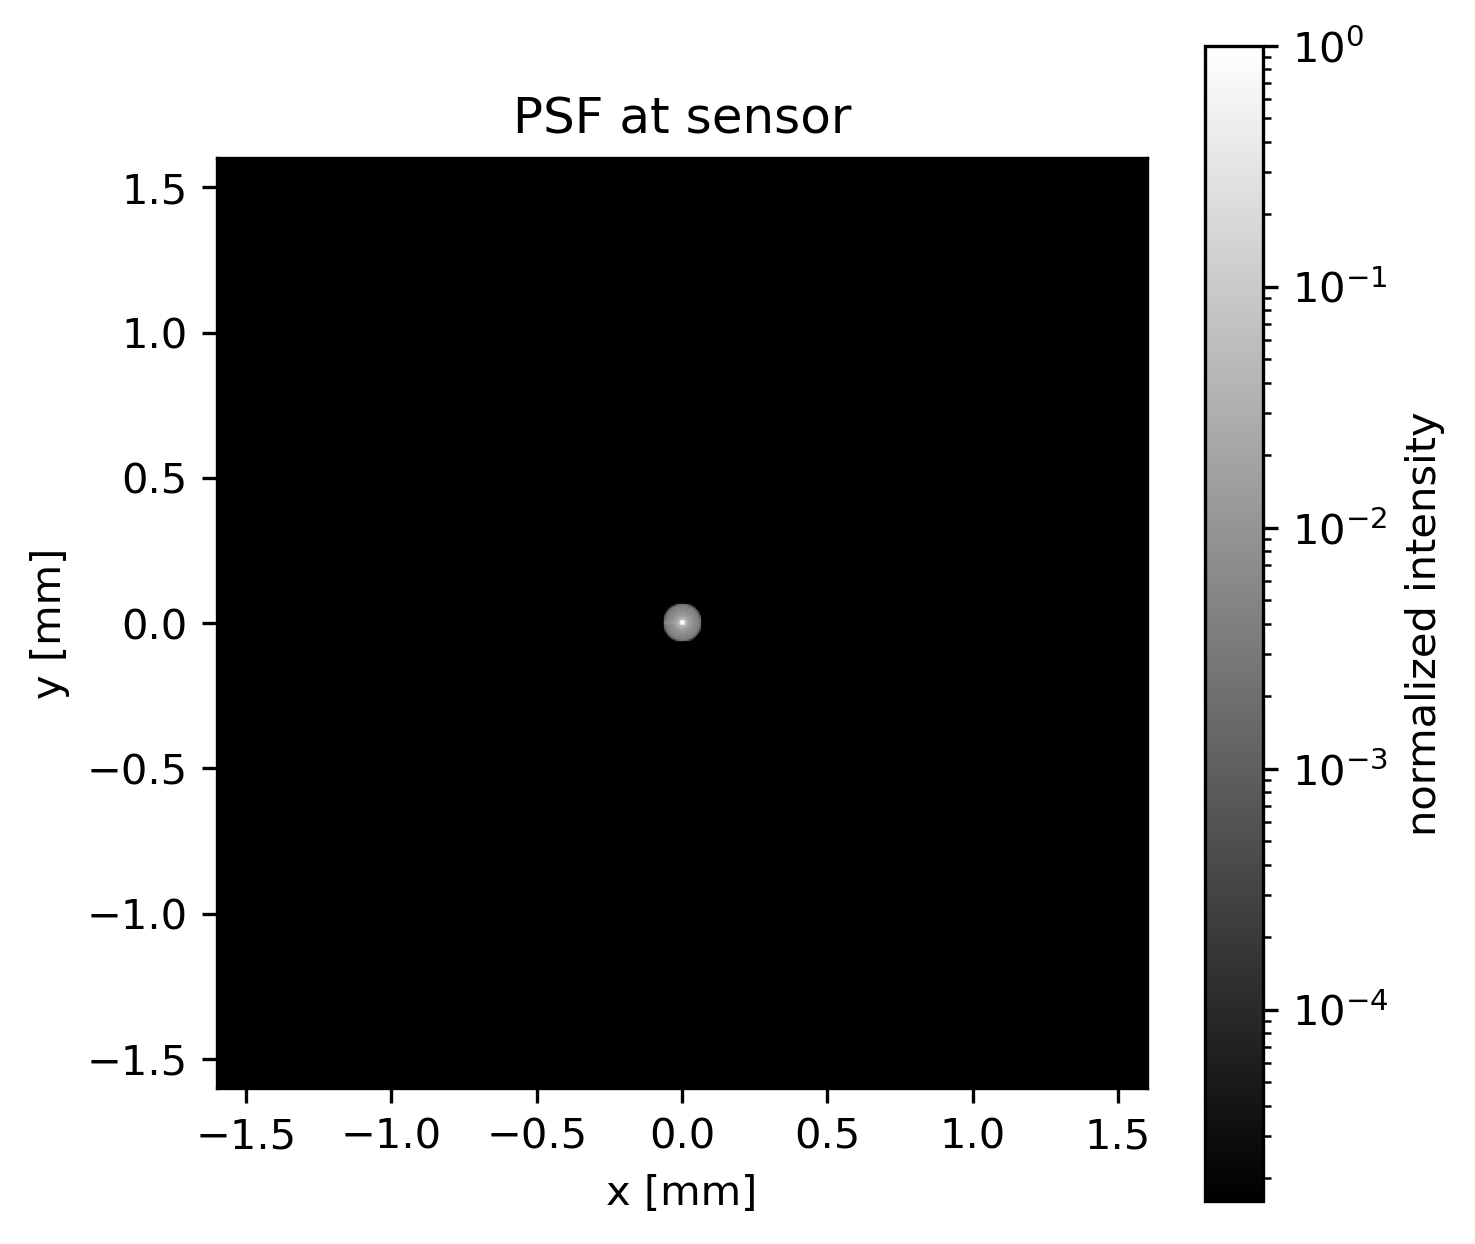
\includegraphics[width=\linewidth,keepaspectratio]{sweep_N/biconvex_psf_3200_log.png} &
			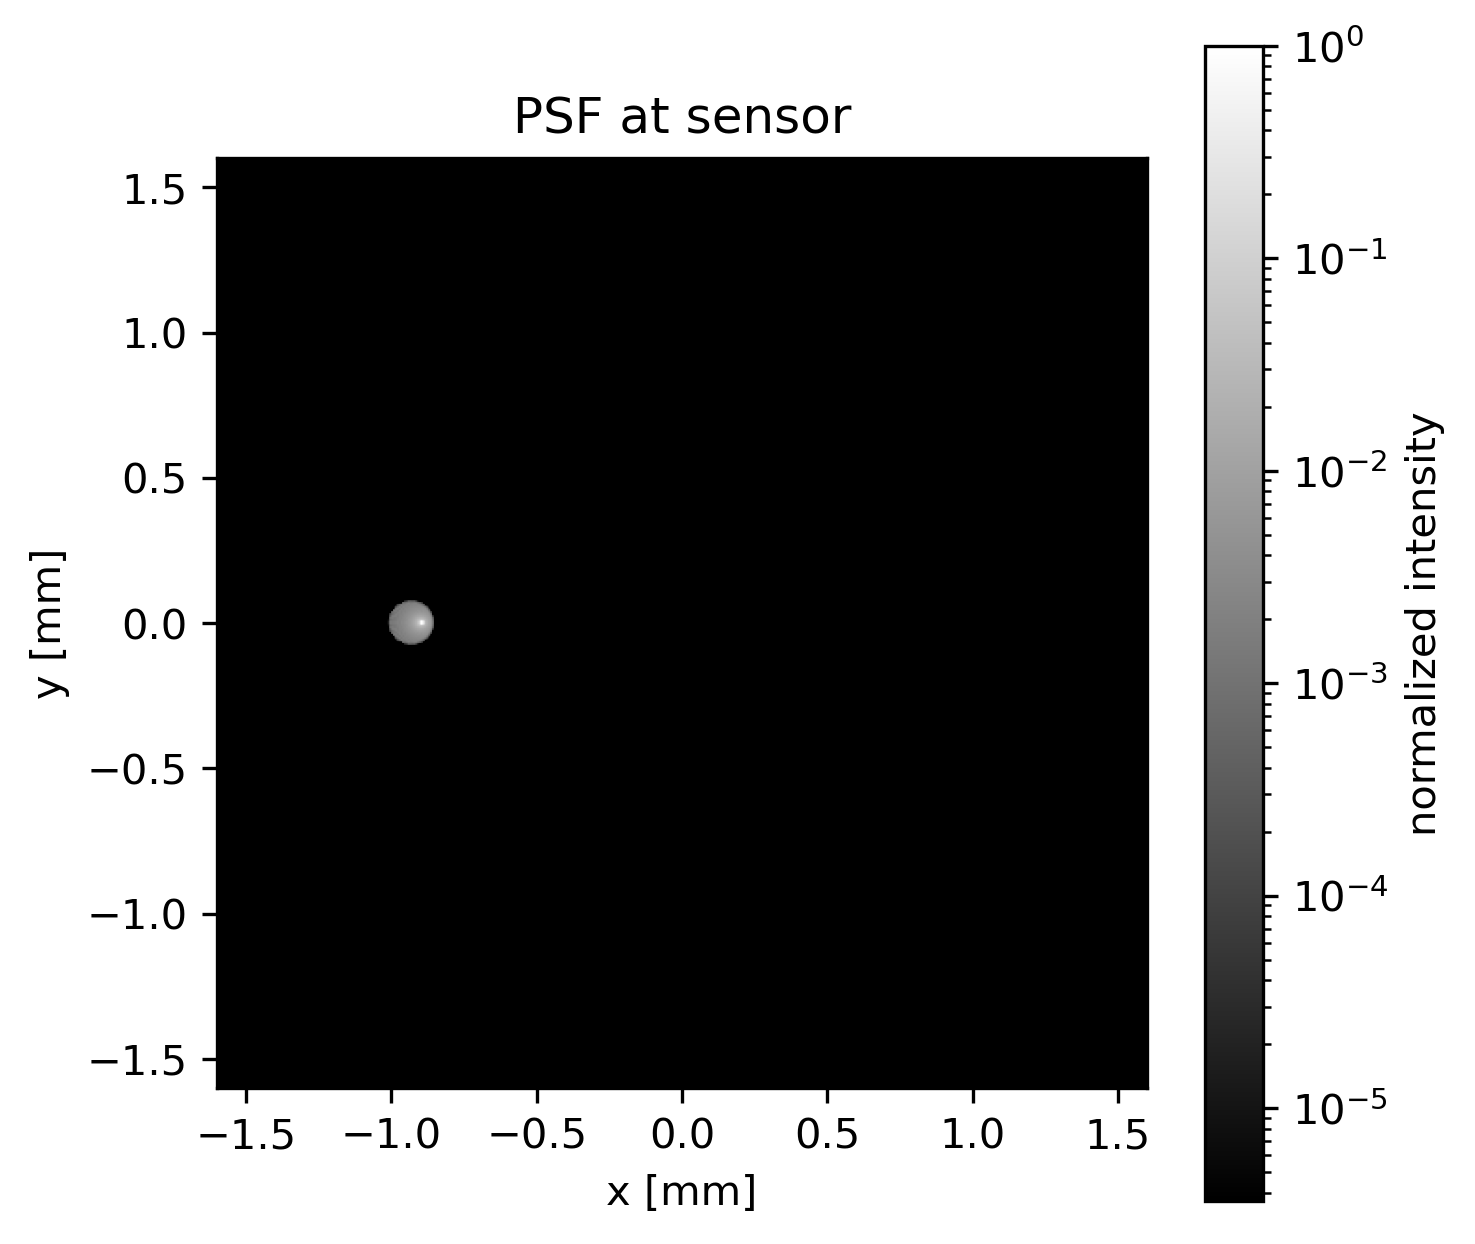
\includegraphics[width=\linewidth,keepaspectratio]{offaxis/biconvex_psf_35.00_log.png} \\
			\bottomrule
		\end{tabular}
		\caption{PSF vs. field offset (biconvex).}
	\end{table}
	
	\begin{figure}[H]
		\centering
		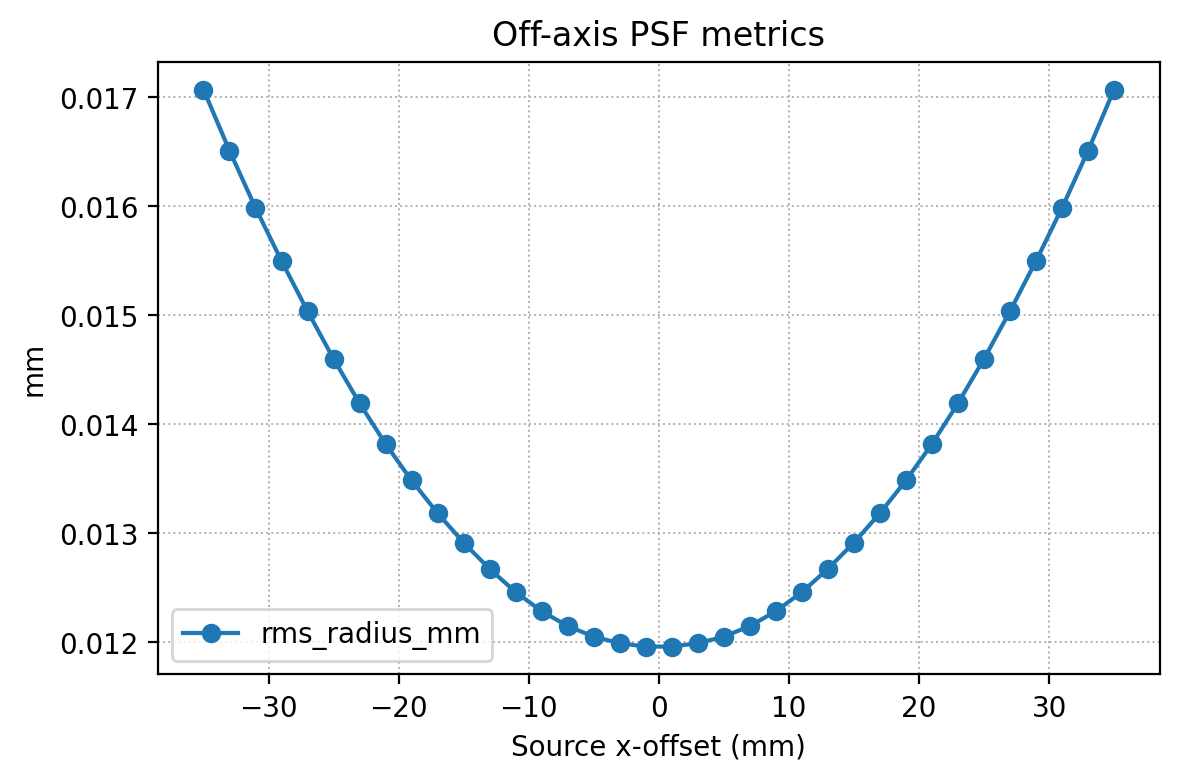
\includegraphics[width=\linewidth]{offaxis/metrics_vs_x_off_mm.png}
		\caption{RMS vs. field offset.}
	\end{figure}
	
	\textbf{Observation}: As the source moves off-axis, the PSF centroid shifts roughly linearly with field; core size stays nearly constant for small offsets, with mild coma/asymmetry at larger field.
	
	\subsection{Discussion and Qualitative Analysis}\label{discussion}
	
	\subsubsection*{Sampling and Aliasing}
	
	With small \(N\), the PSF shows speckle-like noise due to non-uniform pupil mapping; as \(N \gtrsim 1600\), RMS and EE50 stabilize and the PSF becomes smooth.
	Mitigations: increase \(N\); average multiple seeds; sample uniformly on the pupil.
	
	\subsubsection*{Off-Axis Source}
	
	Off-axis increases centroid shift and introduces coma/astigmatism at large field; best-focus distance varies mildly across field, indicating slight field curvature.
	A more complex lens group can suppress these effects.
	
	\subsubsection*{Wavelength Dependence (Chromatic Aberration)}
	
	With BK7 dispersion, \(n(\lambda)\) decreases with \(\lambda\); effective focal length increases with \(\lambda\).
	Thus a fixed sensor plane cannot be perfect for all wavelengths (blue focuses in front; red behind).
	
	\subsubsection*{Aperture Effect (f-number)}
	
	As OD increases from f/16 to f/2:
	EE50 remains nearly constant at small apertures;
	RMS grows at large apertures due to spherical aberration and coma.
	This reflects a brightness--sharpness trade-off.
	
	\subsubsection*{Through-Focus Behavior}
	
	Sweeping \(D_2\) shows smooth degradation away from best focus (\SI{20.5}{mm}); curves are slightly asymmetric and steeper for larger apertures, matching expectations for residual spherical terms.
	
	\subsection{Algorithmic Correction of Aberrations}
	
	Aberrations (defocus, spherical, coma, astigmatism) broaden PSF and reduce contrast. Modeling as a spatially varying PSF \(h(x,y)\), we compare classical vs. learning-based:
	\begin{table}[H]
		\centering
		\caption{Classical deconvolution vs. neural approaches}
		\begin{tabular}{p{0.18\linewidth} p{0.36\linewidth} p{0.36\linewidth}}
			\toprule
			\textbf{Aspect} & \textbf{Classical Deconvolution} & \textbf{Neural Network Approach}\\
			\midrule
			Principle & Linear inversion (e.g., Wiener, RL) with known PSF & Data-driven mapping from blurred to sharp \\
			Pros & Interpretable; predictable; no training data & Handles complex/chromatic/field-dependent aberrations; flexible \\
			Cons & Sensitive to noise/PSF mismatch; non-stationary PSF is hard & Needs data; potential overfitting \\
			Best use & Mild blur, stationary PSF & Complex scenarios, data-rich pipelines \\
			\bottomrule
		\end{tabular}
	\end{table}
	
	\subsection{Model Refinement and Efficiency}
	
	\textbf{Physical accuracy:} include diffraction; model sensor pixel response (e.g., microlens/MTF); consider material tolerances (temperature).\\
	\textbf{Computation:} vectorize intersections; enable GPU acceleration.\\
	\textbf{Function:} extend to scene rendering.
	
	\section*{Conclusion}
	
	The simulator reproduces key behaviors of the Thorlabs LB1761 singlet and the Double-Gauss configuration. Major outcomes:
	\begin{itemize}
		\item \textbf{Functional:} PSF metrics (RMS, EE50); even-grid alignment fix; sampling functions by object distance; \texttt{build\_lens()}; modular structure; unit tests.
		\item \textbf{Validated optics:} Correct Snell refraction and intersections; PSF metrics converge for \(N \ge 1600\); expected trends for wavelength, focus, aperture, and field.
	\end{itemize}
	
	\subsection*{Extra (Double-Gaussian results)}\label{extra-double-gaussian}
	
	We repeat wavelength and off-axis sweeps on a Double-Gauss (aperture \(\approx f/4\)).
	
	\paragraph{Wavelength sweep.}%
	\begin{figure}[H]
		\centering
		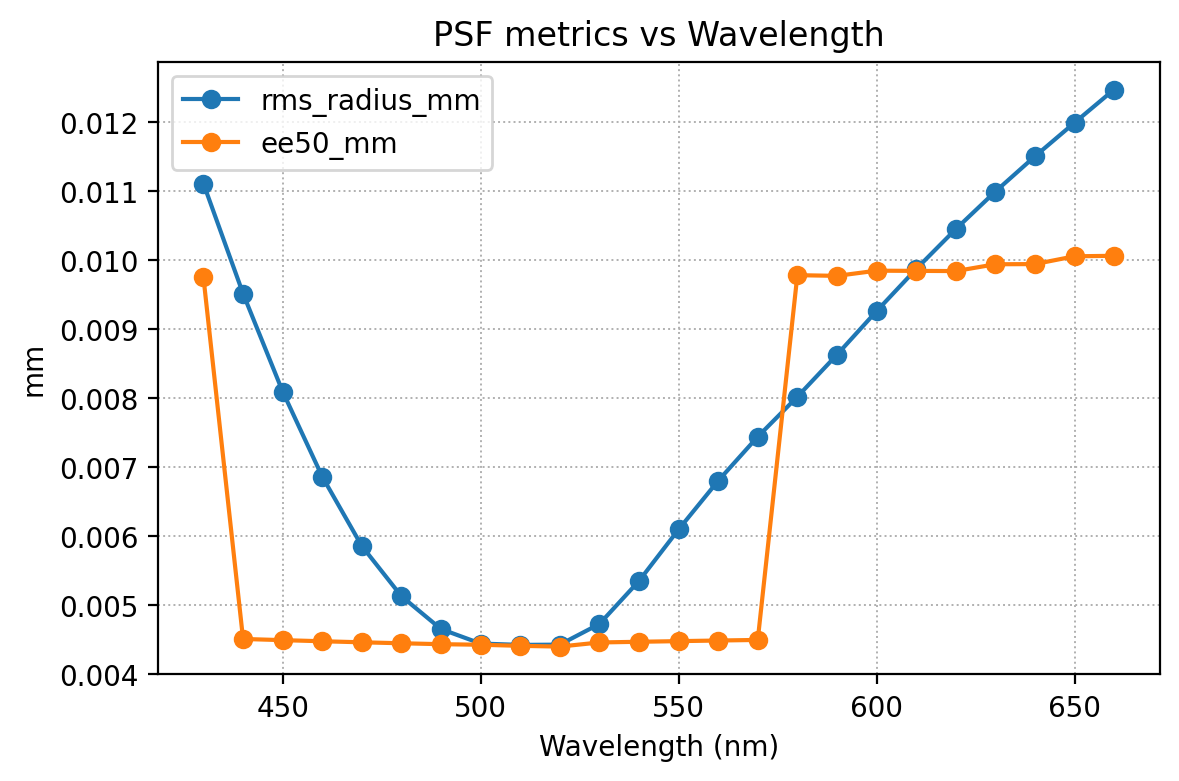
\includegraphics[width=\linewidth]{sweep_lambda/metrics_vs_lambda_nm.png}
		\caption{Double-Gauss: metrics vs. wavelength.}
	\end{figure}
	
	\paragraph{Off-axis sweep.}%
	\begin{table}[H]
		\centering
		\begin{tabular}{>{\centering\arraybackslash}m{0.31\linewidth} >{\centering\arraybackslash}m{0.31\linewidth} >{\centering\arraybackslash}m{0.31\linewidth}}
			\toprule
			Off-axis = \(-\)35 mm & Off-axis = \(-\)1 mm & Off-axis = 35 mm \\
			\midrule
			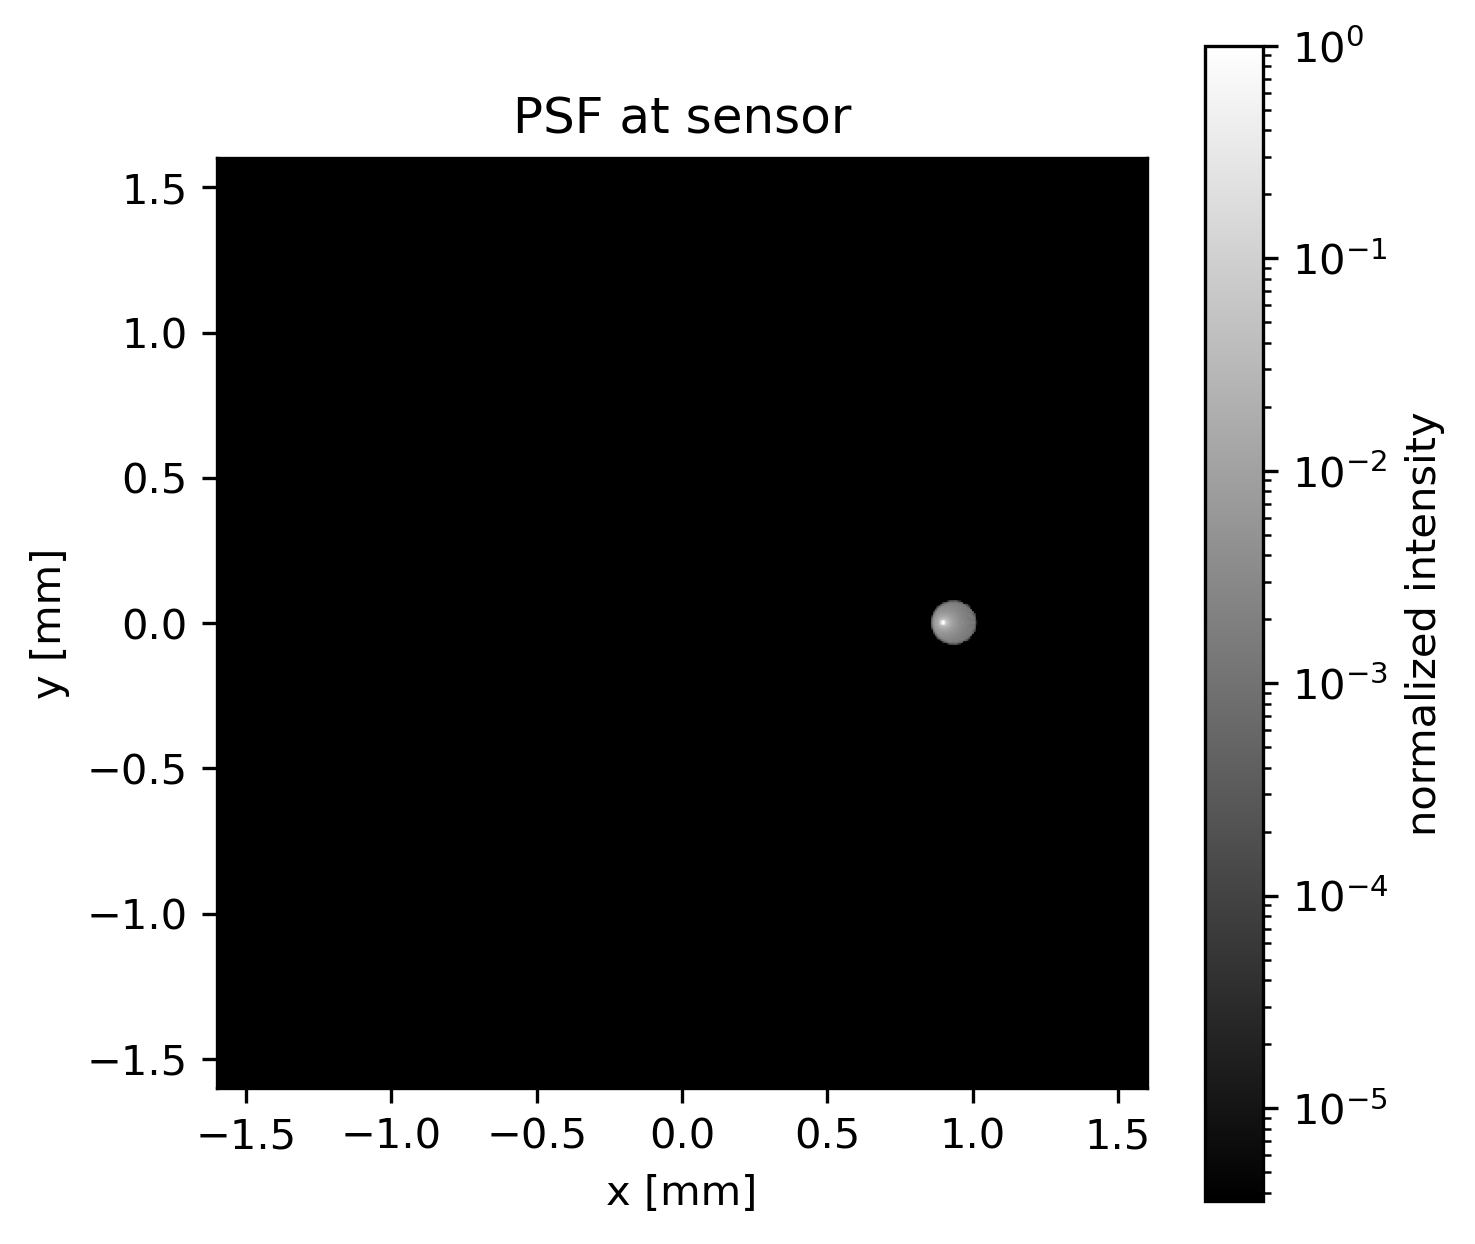
\includegraphics[width=\linewidth,keepaspectratio]{offaxis/biconvex_psf_-35.00_log.png} &
			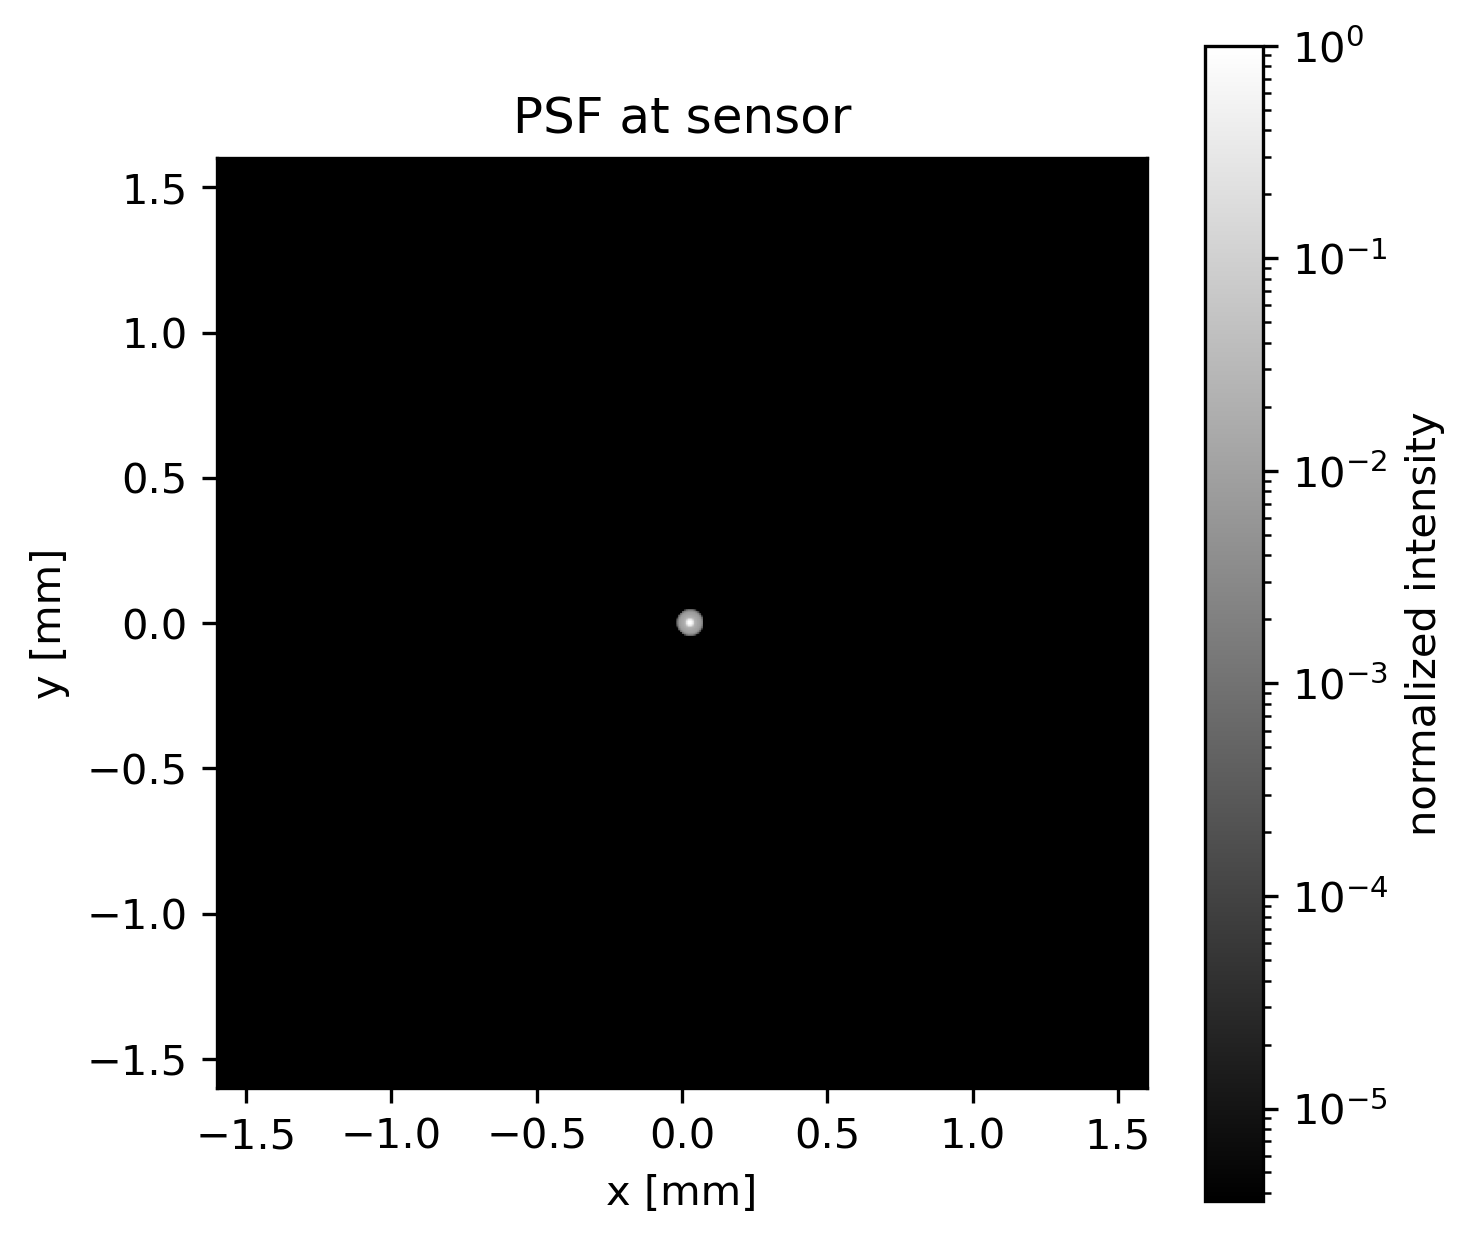
\includegraphics[width=\linewidth,keepaspectratio]{offaxis/biconvex_psf_-1.00_log.png} &
			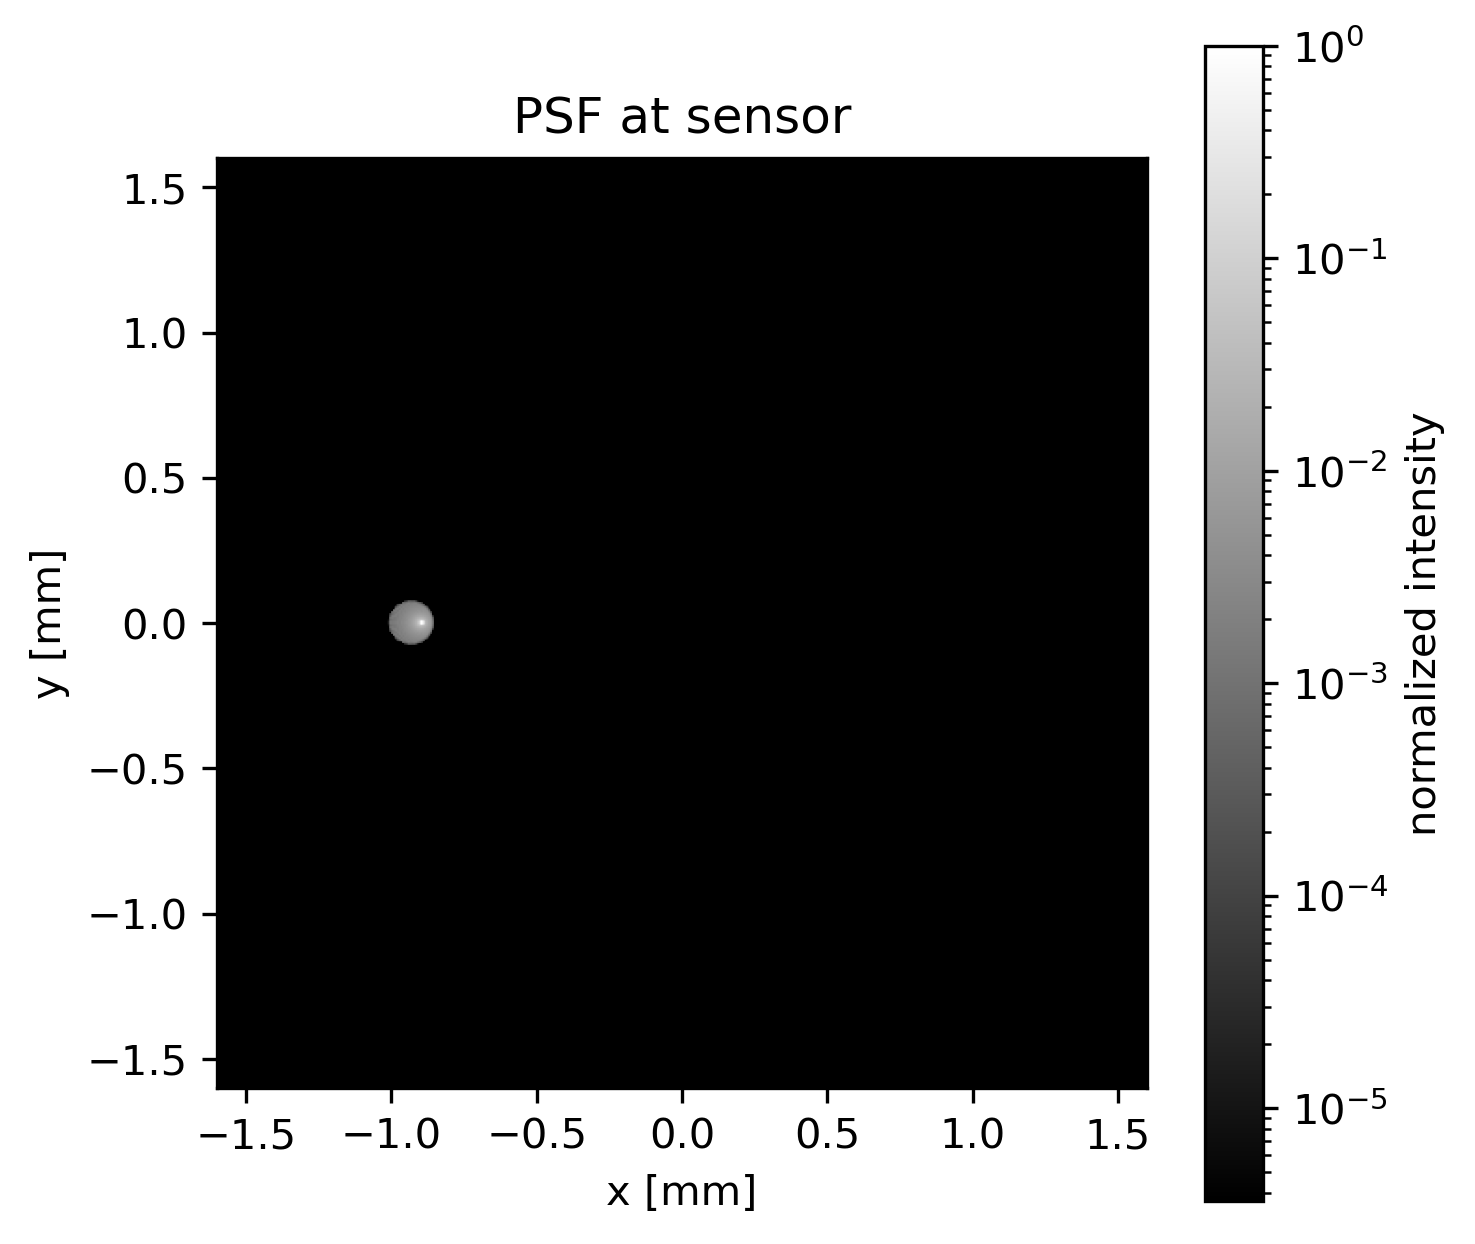
\includegraphics[width=\linewidth,keepaspectratio]{offaxis/biconvex_psf_35.00_log.png} \\
			\bottomrule
		\end{tabular}
		\caption{PSF vs. field offset (Double-Gauss).}
	\end{table}
	
	\textbf{Observation}: With improved lens design, artifacts such as coma and other aberrations are significantly reduced, yielding better focus consistency across wavelengths---especially evident in the Double-Gauss design.
	
\end{document}
